\documentclass[10pt,]{krantz}
\usepackage{lmodern}
\usepackage{amssymb,amsmath}
\usepackage{ifxetex,ifluatex}
\usepackage{fixltx2e} % provides \textsubscript
\ifnum 0\ifxetex 1\fi\ifluatex 1\fi=0 % if pdftex
  \usepackage[T1]{fontenc}
  \usepackage[utf8]{inputenc}
\else % if luatex or xelatex
  \ifxetex
    \usepackage{mathspec}
  \else
    \usepackage{fontspec}
  \fi
  \defaultfontfeatures{Ligatures=TeX,Scale=MatchLowercase}
\fi
% use upquote if available, for straight quotes in verbatim environments
\IfFileExists{upquote.sty}{\usepackage{upquote}}{}
% use microtype if available
\IfFileExists{microtype.sty}{%
\usepackage{microtype}
\UseMicrotypeSet[protrusion]{basicmath} % disable protrusion for tt fonts
}{}
\usepackage[unicode=true]{hyperref}
\PassOptionsToPackage{usenames,dvipsnames}{color} % color is loaded by hyperref
\hypersetup{
            pdftitle={Gráficos con R},
            colorlinks=true,
            linkcolor=Maroon,
            citecolor=Blue,
            urlcolor=Blue,
            breaklinks=true}
\urlstyle{same}  % don't use monospace font for urls
\usepackage{natbib}
\bibliographystyle{apalike}
\usepackage{color}
\usepackage{fancyvrb}
\newcommand{\VerbBar}{|}
\newcommand{\VERB}{\Verb[commandchars=\\\{\}]}
\DefineVerbatimEnvironment{Highlighting}{Verbatim}{commandchars=\\\{\}}
% Add ',fontsize=\small' for more characters per line
\usepackage{framed}
\definecolor{shadecolor}{RGB}{248,248,248}
\newenvironment{Shaded}{\begin{snugshade}}{\end{snugshade}}
\newcommand{\KeywordTok}[1]{\textcolor[rgb]{0.13,0.29,0.53}{\textbf{{#1}}}}
\newcommand{\DataTypeTok}[1]{\textcolor[rgb]{0.13,0.29,0.53}{{#1}}}
\newcommand{\DecValTok}[1]{\textcolor[rgb]{0.00,0.00,0.81}{{#1}}}
\newcommand{\BaseNTok}[1]{\textcolor[rgb]{0.00,0.00,0.81}{{#1}}}
\newcommand{\FloatTok}[1]{\textcolor[rgb]{0.00,0.00,0.81}{{#1}}}
\newcommand{\ConstantTok}[1]{\textcolor[rgb]{0.00,0.00,0.00}{{#1}}}
\newcommand{\CharTok}[1]{\textcolor[rgb]{0.31,0.60,0.02}{{#1}}}
\newcommand{\SpecialCharTok}[1]{\textcolor[rgb]{0.00,0.00,0.00}{{#1}}}
\newcommand{\StringTok}[1]{\textcolor[rgb]{0.31,0.60,0.02}{{#1}}}
\newcommand{\VerbatimStringTok}[1]{\textcolor[rgb]{0.31,0.60,0.02}{{#1}}}
\newcommand{\SpecialStringTok}[1]{\textcolor[rgb]{0.31,0.60,0.02}{{#1}}}
\newcommand{\ImportTok}[1]{{#1}}
\newcommand{\CommentTok}[1]{\textcolor[rgb]{0.56,0.35,0.01}{\textit{{#1}}}}
\newcommand{\DocumentationTok}[1]{\textcolor[rgb]{0.56,0.35,0.01}{\textbf{\textit{{#1}}}}}
\newcommand{\AnnotationTok}[1]{\textcolor[rgb]{0.56,0.35,0.01}{\textbf{\textit{{#1}}}}}
\newcommand{\CommentVarTok}[1]{\textcolor[rgb]{0.56,0.35,0.01}{\textbf{\textit{{#1}}}}}
\newcommand{\OtherTok}[1]{\textcolor[rgb]{0.56,0.35,0.01}{{#1}}}
\newcommand{\FunctionTok}[1]{\textcolor[rgb]{0.00,0.00,0.00}{{#1}}}
\newcommand{\VariableTok}[1]{\textcolor[rgb]{0.00,0.00,0.00}{{#1}}}
\newcommand{\ControlFlowTok}[1]{\textcolor[rgb]{0.13,0.29,0.53}{\textbf{{#1}}}}
\newcommand{\OperatorTok}[1]{\textcolor[rgb]{0.81,0.36,0.00}{\textbf{{#1}}}}
\newcommand{\BuiltInTok}[1]{{#1}}
\newcommand{\ExtensionTok}[1]{{#1}}
\newcommand{\PreprocessorTok}[1]{\textcolor[rgb]{0.56,0.35,0.01}{\textit{{#1}}}}
\newcommand{\AttributeTok}[1]{\textcolor[rgb]{0.77,0.63,0.00}{{#1}}}
\newcommand{\RegionMarkerTok}[1]{{#1}}
\newcommand{\InformationTok}[1]{\textcolor[rgb]{0.56,0.35,0.01}{\textbf{\textit{{#1}}}}}
\newcommand{\WarningTok}[1]{\textcolor[rgb]{0.56,0.35,0.01}{\textbf{\textit{{#1}}}}}
\newcommand{\AlertTok}[1]{\textcolor[rgb]{0.94,0.16,0.16}{{#1}}}
\newcommand{\ErrorTok}[1]{\textcolor[rgb]{0.64,0.00,0.00}{\textbf{{#1}}}}
\newcommand{\NormalTok}[1]{{#1}}
\usepackage{longtable,booktabs}
\usepackage{graphicx,grffile}
\makeatletter
\def\maxwidth{\ifdim\Gin@nat@width>\linewidth\linewidth\else\Gin@nat@width\fi}
\def\maxheight{\ifdim\Gin@nat@height>\textheight\textheight\else\Gin@nat@height\fi}
\makeatother
% Scale images if necessary, so that they will not overflow the page
% margins by default, and it is still possible to overwrite the defaults
% using explicit options in \includegraphics[width, height, ...]{}
\setkeys{Gin}{width=\maxwidth,height=\maxheight,keepaspectratio}
\IfFileExists{parskip.sty}{%
\usepackage{parskip}
}{% else
\setlength{\parindent}{0pt}
\setlength{\parskip}{6pt plus 2pt minus 1pt}
}
\setlength{\emergencystretch}{3em}  % prevent overfull lines
\providecommand{\tightlist}{%
  \setlength{\itemsep}{0pt}\setlength{\parskip}{0pt}}
\setcounter{secnumdepth}{5}
% Redefines (sub)paragraphs to behave more like sections
\ifx\paragraph\undefined\else
\let\oldparagraph\paragraph
\renewcommand{\paragraph}[1]{\oldparagraph{#1}\mbox{}}
\fi
\ifx\subparagraph\undefined\else
\let\oldsubparagraph\subparagraph
\renewcommand{\subparagraph}[1]{\oldsubparagraph{#1}\mbox{}}
\fi
\usepackage{booktabs}
\usepackage[spanish]{babel}
\decimalpoint
\selectlanguage{spanish}

% Comandos para escribir nombres de paquetes, programas y codigos
\newcommand{\pkg}[1]{{\normalfont\fontseries{b}\selectfont #1}}
\let\proglang=\textsf
\let\code=\texttt


\usepackage{booktabs}
\usepackage{longtable}
\usepackage[bf,singlelinecheck=off]{caption}

\usepackage{framed,color}
\definecolor{shadecolor}{RGB}{248,248,248}

\renewcommand{\textfraction}{0.05}
\renewcommand{\topfraction}{0.8}
\renewcommand{\bottomfraction}{0.8}
\renewcommand{\floatpagefraction}{0.75}

\renewenvironment{quote}{\begin{VF}}{\end{VF}}
\let\oldhref\href
\renewcommand{\href}[2]{#2\footnote{\url{#1}}}

\ifxetex
  \usepackage{letltxmacro}
  \setlength{\XeTeXLinkMargin}{1pt}
  \LetLtxMacro\SavedIncludeGraphics\includegraphics
  \def\includegraphics#1#{% #1 catches optional stuff (star/opt. arg.)
    \IncludeGraphicsAux{#1}%
  }%
  \newcommand*{\IncludeGraphicsAux}[2]{%
    \XeTeXLinkBox{%
      \SavedIncludeGraphics#1{#2}%
    }%
  }%
\fi

\makeatletter
\newenvironment{kframe}{%
\medskip{}
\setlength{\fboxsep}{.8em}
 \def\at@end@of@kframe{}%
 \ifinner\ifhmode%
  \def\at@end@of@kframe{\end{minipage}}%
  \begin{minipage}{\columnwidth}%
 \fi\fi%
 \def\FrameCommand##1{\hskip\@totalleftmargin \hskip-\fboxsep
 \colorbox{shadecolor}{##1}\hskip-\fboxsep
     % There is no \\@totalrightmargin, so:
     \hskip-\linewidth \hskip-\@totalleftmargin \hskip\columnwidth}%
 \MakeFramed {\advance\hsize-\width
   \@totalleftmargin\z@ \linewidth\hsize
   \@setminipage}}%
 {\par\unskip\endMakeFramed%
 \at@end@of@kframe}
\makeatother

\renewenvironment{Shaded}{\begin{kframe}}{\end{kframe}}

\usepackage{makeidx}
\makeindex

\urlstyle{tt}

\usepackage{amsthm}
\makeatletter
\def\thm@space@setup{%
  \thm@preskip=8pt plus 2pt minus 4pt
  \thm@postskip=\thm@preskip
}
\makeatother

\frontmatter

\title{Gráficos con R}
\author{Juan Carlos Correa Morales\\
Freddy Hernández Barajas}
\date{2017-01-19}

\let\BeginKnitrBlock\begin \let\EndKnitrBlock\end
\begin{document}
\maketitle

% you may need to leave a few empty pages before the dedication page

%\cleardoublepage\newpage\thispagestyle{empty}\null
%\cleardoublepage\newpage\thispagestyle{empty}\null
%\cleardoublepage\newpage
\thispagestyle{empty}

\begin{center}

Gracias a Dios por todo lo que me ha dado.

%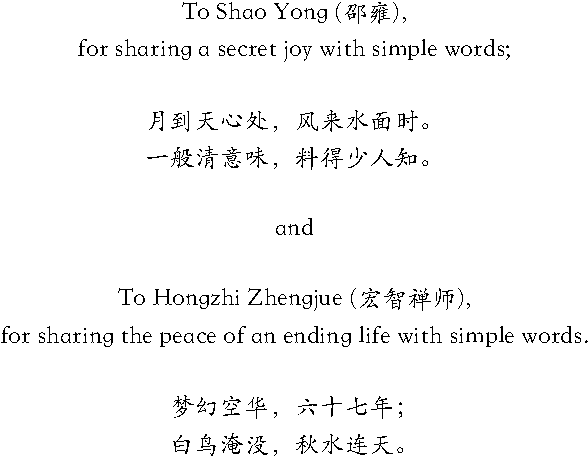
\includegraphics{images/dedication.pdf}
\end{center}

\setlength{\abovedisplayskip}{-5pt}
\setlength{\abovedisplayshortskip}{-5pt}

{
\hypersetup{linkcolor=black}
\setcounter{tocdepth}{2}
\tableofcontents
}
\listoftables
\listoffigures
\chapter*{Prefacio}\label{prefacio}


Este libro fue creado con la intención de ayudar a los estudiantes de
pregrado, especialización, maestría e investigadores a crear gráficos
estadísticos con las herramientas básicas de \proglang{R}. Como
complemento, recomendamos a los lectores el libro
\citet{hernandez_usuga} que muestra cómo usar \proglang{R} para realizar
diversos procedimiento estadísticos.

\section*{¿Por qué leer este libro?}\label{por-que-leer-este-libro}


Este libro es importante porque \ldots{}

\section*{Estructura del libro}\label{estructura-del-libro}


En el capítulo \ref{intro} se presenta una introducción breve de
\proglang{R}, sus orígenes, la instalación, tipos de objetos y una guía
de estilo para escribir en \proglang{R}.

\section*{Software information and
conventions}\label{software-information-and-conventions}


Para realizar este libro usamos los paquetes \textbf{knitr}\index{knitr}
\citep{xie2015} y \textbf{bookdown}\index{bookdown} \citep{R-bookdown}.

Package names are in bold text (e.g., \textbf{rmarkdown}), and inline
code and filenames are formatted in a typewriter font (e.g.,
\texttt{knitr::knit(\textquotesingle{}foo.Rmd\textquotesingle{})}).
Function names are followed by parentheses (e.g.,
\texttt{bookdown::render\_book()}).

En todo el libro se presentarán códigos que el lector puede copiar y
pegar en su consola de \proglang{R} para obtener los mismos resultados
aquí presentados. Los códigos se destacan en una caja de color beis (o
beige) similar a la mostrada a continuación.

\begin{Shaded}
\begin{Highlighting}[]
\DecValTok{4} \NormalTok{+}\StringTok{ }\DecValTok{6}
\NormalTok{a <-}\StringTok{ }\KeywordTok{c}\NormalTok{(}\DecValTok{1}\NormalTok{, }\DecValTok{5}\NormalTok{, }\DecValTok{6}\NormalTok{)}
\DecValTok{5} \NormalTok{*}\StringTok{ }\NormalTok{a}
\DecValTok{1}\NormalTok{:}\DecValTok{10}
\end{Highlighting}
\end{Shaded}

Los resultados o salidas obtenidos de cualquier código se destacan con
dos símbolos de númeral (\texttt{\#\#}) al inicio de cada línea o
renglón, esto quiere decir que todo lo que inicie con \texttt{\#\#} son
resultados obtenidos y \textbf{NO} los debe copiar. Abajo se muestran
los resultados obtenidos luego de correr el código anterior.

\begin{verbatim}
## [1] 10
\end{verbatim}

\begin{verbatim}
## [1]  5 25 30
\end{verbatim}

\begin{verbatim}
##  [1]  1  2  3  4  5  6  7  8  9 10
\end{verbatim}

\section*{Agradecimientos}\label{agradecimientos}


Agradecemos a nuestros estudiantes, profesores y colegas que han leído
el manuscrito y se han tomado el trabajo de escribirnos dándonos sus
sugerencias y comentarios para mejorar continuamente este material.

\BeginKnitrBlock{flushright}
Juan Carlos Correa Morales

Freddy Hernández Barajas
\EndKnitrBlock{flushright}

\chapter*{Sobre los autores}\label{sobre-los-autores}


Juan Carlos Correa Morales es profesor asociado de la Universidad
Nacional de Colombia adscrito a la Escuela de Estadística de la Facultad
de Ciencias.

\href{mailto:jccorreamorales@gmail.com}{\nolinkurl{jccorreamorales@gmail.com}}

Freddy Hernández Barajas es profesor asistente de la Universidad
Nacional de Colombia adscrito a la Escuela de Estadística de la Facultad
de Ciencias.

\href{mailto:fhernanb@unal.edu.co}{\nolinkurl{fhernanb@unal.edu.co}}

\mainmatter

\chapter{\texorpdfstring{Introducción
\label{intro}}{Introducción }}\label{introduccion}

\section{Orígenes} \label{sec:origenes}

\proglang{R} es un lenguaje de programación usado para realizar
procedimientos estadísticos y gráficos de alto nivel, este lenguaje fue
creado en 1993 por los profesores e investigadores Robert Gentleman y
Ross Ihaka. Inicialmente el lenguaje se usó para apoyar los cursos que
tenían a su cargo los profesores, pero luego de ver la utilidad de la
herramienta desarrollada, decidieron colocar copias de \proglang{R} en
StatLib. A partir de 1995 el código fuente de \proglang{R} está
disponible bajo licencia GNU GPL para sistemas operativos Windows,
Macintosh y distribuciones Unix/Linux. La comunidad de usuarios de
\proglang{R} en el mundo es muy grande y los usuarios cuentan con
diferentes espacios para interactuar, a continuación una lista no
exhaustiva de los sitios más populares relacionados con \proglang{R}:

\begin{itemize}
\tightlist
\item
  \href{https://www.r-bloggers.com/}{Rbloggers}.
\item
  \href{http://r-es.org/}{Comunidad hispana de \proglang{R}}.
\item
  \href{http://r.789695.n4.nabble.com/}{Nabble}.
\item
  \href{http://r-br.2285057.n4.nabble.com/}{Foro en portugués}.
\item
  \href{http://stackoverflow.com/questions/tagged/r}{Stackoverflow}.
\item
  \href{http://stats.stackexchange.com/questions/tagged/r}{Cross
  Validated}.
\item
  \href{https://stat.ethz.ch/mailman/listinfo/r-help}{\proglang{R}-Help
  Mailing List}.
\item
  \href{http://blog.revolutionanalytics.com/}{Revolutions}.
\item
  \href{https://www.r-statistics.com/}{\proglang{R}-statistics blog}.
\item
  \href{https://rdatamining.wordpress.com/}{RDataMining}.
\end{itemize}

\begin{figure}

{\centering 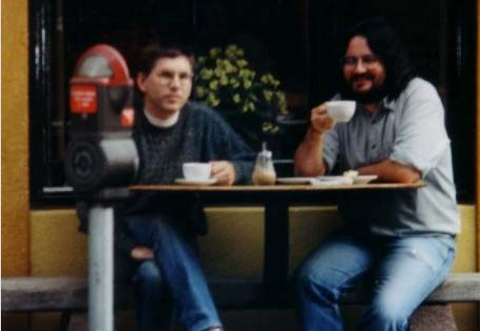
\includegraphics[width=2.4in]{images/Robert_Roos} 

}

\caption{Robert Gentleman (izquierda) y Ross Ihaka (derecha) creadores de R.}\label{fig:unnamed-chunk-4}
\end{figure}

\section{Descarga e instalación} \label{sec:descarga}

Para realizar la instalación de \proglang{R} usted debe visitar la
página del CRAN (\textit{Comprehensive R Archive Network}) disponible en
este \href{https://cran.r-project.org/}{enlace}. Una vez ingrese a la
página encontrará un cuadro similar al mostrado en la Figura
\ref{fig:cran} donde aparecen los enlaces de la instalación para los
sistemas operativos Linux, Mac y Windows.

\begin{figure}

{\centering 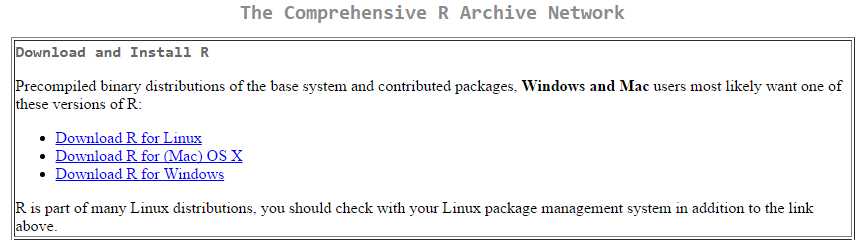
\includegraphics[width=4.54in]{images/cran} 

}

\caption{Página del Cran.}\label{fig:cran}
\end{figure}

Supongamos que se desea instalar \proglang{R} en Windows, para esto se
debe dar clic sobre el hiperenlace
\textcolor{BurntOrange}{Download R for Windows} de la Figura
\ref{fig:cran}. Una vez hecho esto se abrirá una página con el contenido
mostrado en la Figura \ref{fig:inst1}. Una vez ingrese a esa nueva
página usted debe dar clic sobre el hiperenlace
\textcolor{BurntOrange}{install R for the first time} como es señalado
por la flecha roja en la Figura \ref{fig:inst1}.

\begin{figure}

{\centering 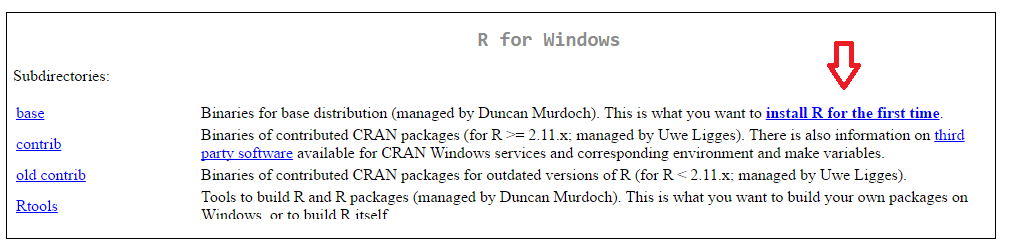
\includegraphics[width=5.31in]{images/instalacion1} 

}

\caption{Página de instalación para la primera ocasión.}\label{fig:inst1}
\end{figure}

Luego de esto se abrirá otra página con un encabezado similar al
mostrado en la Figura \ref{fig:inst2}, al momento de capturar la figura
la versión actual de \proglang{R} era 3.2.5 pero seguramente en este
momento usted tendrá disponible una versión actualizada. Una vez allí
uste debe dar clic sobre
\textcolor{BurntOrange}{Download R 3.2.5 for Windows} como es señalado
por la flecha verde. Luego de esto se descargará el instalador
\proglang{R} en el computador el cual deberá ser instalado con las
opciones que vienen por defecto.

\begin{figure}

{\centering 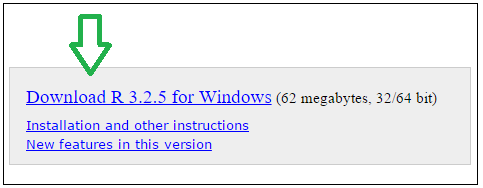
\includegraphics[width=2.54in]{images/instalacion2} 

}

\caption{Página de descarga.}\label{fig:inst2}
\end{figure}

Se recomienda observar el siguiente video didáctico de instalación de
\proglang{R} disponible en este
\href{http://tinyurl.com/jd7b9ks}{enlace} para facilitar la tarea de
instalación.

\section{Apariencia del programa} \label{sec:apariencia}

Una vez que esté instalado \proglang{R} en su computador, usted podrá
acceder a él por la lista de programas o por medio del acceso directo
que quedó en el escritorio, en la Figura \ref{fig:rlogo} se muestra la
apariencia del acceso directo para ingresar a \proglang{R}.

\begin{figure}

{\centering 
\includegraphics[width=1.14in]{images/rlogo} 

}

\caption{Apariencia del acceso directo para ingresar a R.}\label{fig:rlogo}
\end{figure}

Al abrir \proglang{R} aparecerá en la pantalla de su computador algo
similar a lo que está en la Figura \ref{fig:pantalla}. La ventana
izquierda se llama consola y es donde se ingresan las instrucciones, una
vez que se construye un gráfico se activa otra ventana llamada ventana
gráfica. Cualquier usuario puede modificar la posición y tamaños de
estas ventanas, puede cambiar el tipo y tamaño de las letras en la
consola, para hacer esto se deben explorar las opciones de
\textit{editar} en la barra de herramientas.

\begin{figure}

{\centering 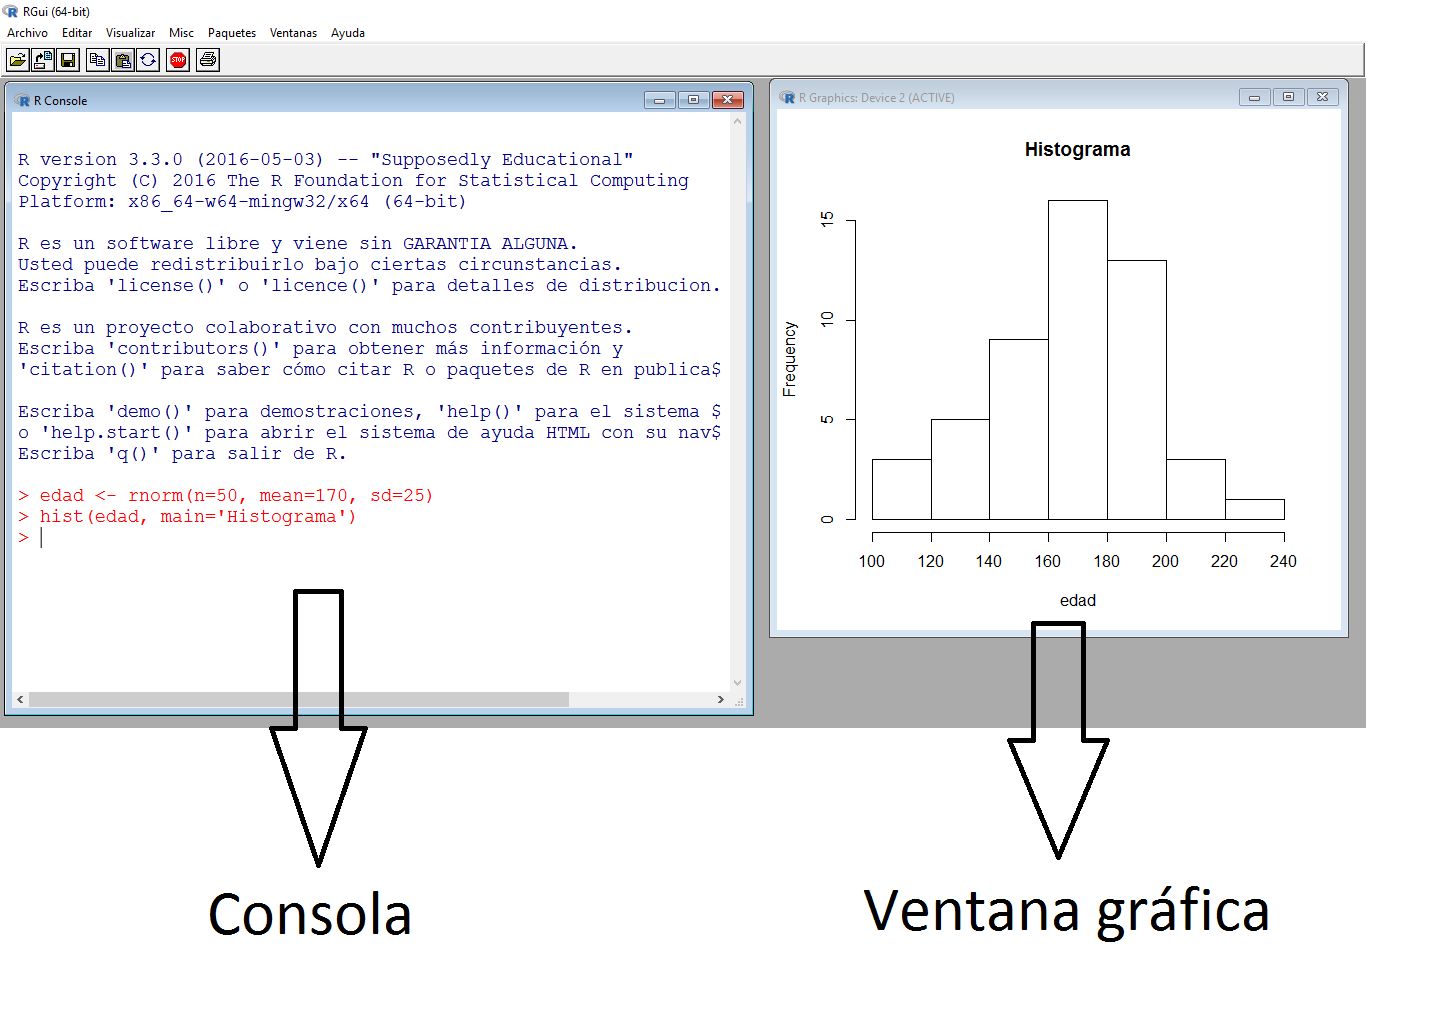
\includegraphics[width=3.6in]{images/Rpantallazo} 

}

\caption{Apariencia de R.}\label{fig:pantalla}
\end{figure}

\section{Tipos de objetos} \label{sec:objetos}

En \proglang{R} existen varios tipos de objectos \index{objetos} que
permiten que el usuario pueda almacenar la información para realizar
procedimientos estadísticos y gráficos. Los principales objetos en
\proglang{R} son vectores, matrices, arreglos, marcos de datos y listas.
A continuación se presentan las características de estos objetos y la
forma para crearlos.

\subsection{Vectores}

Los vectores \index{vectores} son arreglos ordenados en los cuales se
puede almacenar información de tipo numérico (variable cuantitativa),
alfanumérico (variable cualitativa) o lógico (\texttt{TRUE} o
\texttt{FALSE}), pero no mezclas de éstos. La función de \proglang{R}
para crear un vector es \texttt{c()} y que significa concatenar; dentro
de los paréntesis de esta función se ubica la información a almacenar.
Una vez construído el vector se acostumbra a etiquetarlo con un nombre
corto y representativo de la información que almacena, la asignación se
hace por medio del operador \texttt{\textless{}-} entre el nombre y el
vector.

A continuación se presenta un ejemplo de cómo crear tres vectores que
contienen las respuestas de cinco personas a tres preguntas que se les
realizaron.

\begin{Shaded}
\begin{Highlighting}[]
\NormalTok{edad <-}\StringTok{ }\KeywordTok{c}\NormalTok{(}\DecValTok{15}\NormalTok{, }\DecValTok{19}\NormalTok{, }\DecValTok{13}\NormalTok{, }\OtherTok{NA}\NormalTok{, }\DecValTok{20}\NormalTok{)}
\NormalTok{deporte <-}\StringTok{ }\KeywordTok{c}\NormalTok{(}\OtherTok{TRUE}\NormalTok{, }\OtherTok{TRUE}\NormalTok{, }\OtherTok{NA}\NormalTok{, }\OtherTok{FALSE}\NormalTok{, }\OtherTok{TRUE}\NormalTok{)}
\NormalTok{comic.fav <-}\StringTok{ }\KeywordTok{c}\NormalTok{(}\OtherTok{NA}\NormalTok{, }\StringTok{'Superman'}\NormalTok{, }\StringTok{'Batman'}\NormalTok{, }\OtherTok{NA}\NormalTok{, }\StringTok{'Batman'}\NormalTok{)}
\end{Highlighting}
\end{Shaded}

El vector \texttt{edad} es un vector cuantitativo y contiene las edades
de las 5 personas. En la cuarta posición del vector se colocó el símbolo
\texttt{NA} que significa \textit{Not Available} debido a que no se
registró la edad para esa persona. Al hacer una asignación se acostumbra
a dejar un espacio antes y después del operador \texttt{\textless{}-} de
asignación. El segundo vector es llamado \texttt{deporte} y es un vector
lógico que almacena las respuestas a la pregunta de si la persona
practica deporte, nuevamente aquí hay un \texttt{NA} para la tercera
persona. El último vector \texttt{comic.fav} contiene la información del
cómic favorito de cada persona, como esta variable es cualitativa es
necesario usar las comillas
\texttt{\textquotesingle{}\ \textquotesingle{}} para encerrar las
respuestas. Cuando se usa \texttt{NA} para representar una información
\textit{Not Available} NO SE DEBEN usar las comillas
\texttt{\textquotesingle{}\ \textquotesingle{}}.

Nota: es posible usar comillas sencillas
\texttt{\textquotesingle{}foo\textquotesingle{}} o comillas dobles
\texttt{"foo"} para ingresar valores de una variable cualitativa.

Si se desea ver lo que está almacenado en cada uno de estos vectores, se
debe escribir en la consola de \proglang{R} el nombre de uno de los
objetos y luego se presiona la tecla \textit{enter} o \textit{intro}, al
realizar esto lo que se obtiene se muestra a continuación.

\begin{Shaded}
\begin{Highlighting}[]
\NormalTok{edad}
\end{Highlighting}
\end{Shaded}

\begin{verbatim}
## [1] 15 19 13 NA 20
\end{verbatim}

\begin{Shaded}
\begin{Highlighting}[]
\NormalTok{deporte}
\end{Highlighting}
\end{Shaded}

\begin{verbatim}
## [1]  TRUE  TRUE    NA FALSE  TRUE
\end{verbatim}

\begin{Shaded}
\begin{Highlighting}[]
\NormalTok{comic.fav}
\end{Highlighting}
\end{Shaded}

\begin{verbatim}
## [1] NA         "Superman" "Batman"   NA        
## [5] "Batman"
\end{verbatim}

\subsection{Matrices}

Las matrices \index{matrices} son arreglos rectangulares de filas y
columnas con información numérica, alfanumérica o lógica. Para construir
una matriz se usa la función \texttt{matrix(\ )}. Por ejemplo, para
crear una matriz de 4 filas y 5 columnas (de dimensión \(4 \times 5\))
con los primeros 20 números positivos se escribe el código siguiente en
la consola.

\begin{Shaded}
\begin{Highlighting}[]
\NormalTok{mimatriz <-}\StringTok{ }\KeywordTok{matrix}\NormalTok{(}\DataTypeTok{data=}\DecValTok{1}\NormalTok{:}\DecValTok{20}\NormalTok{, }\DataTypeTok{nrow=}\DecValTok{4}\NormalTok{, }\DataTypeTok{ncol=}\DecValTok{5}\NormalTok{, }\DataTypeTok{byrow=}\OtherTok{FALSE}\NormalTok{)}
\end{Highlighting}
\end{Shaded}

El argumento \texttt{data} de la función sirve para indicar los datos
que se van a almacenar en la matriz, los argumentos \texttt{nrow} y
\texttt{ncol} sirven para definir la dimensión de la matriz y por último
el argumento \texttt{byrow} sirve para indicar si la información
contenida en \texttt{data} se debe ingresar por filas o no. Para
observar lo que quedó almacenado en el objeto \texttt{mimatriz} se
escribe en la consola el nombre del objeto seguido de la tecla
\textit{enter} o \textit{intro}.

\begin{Shaded}
\begin{Highlighting}[]
\NormalTok{mimatriz}
\end{Highlighting}
\end{Shaded}

\begin{verbatim}
##      [,1] [,2] [,3] [,4] [,5]
## [1,]    1    5    9   13   17
## [2,]    2    6   10   14   18
## [3,]    3    7   11   15   19
## [4,]    4    8   12   16   20
\end{verbatim}

\subsection{Arreglos}

Un arreglo \index{arreglo} es una matriz de varias dimensiones con
información numérica, alfanumérica o lógica. Para construir una arreglo
se usa la función \texttt{array(\ )}. Por ejemplo, para crear un arreglo
de \(3 \times 4 \times 2\) con las primeras 24 letras minúsculas del
alfabeto se escribe el siguiente código.

\begin{Shaded}
\begin{Highlighting}[]
\NormalTok{miarray <-}\StringTok{ }\KeywordTok{array}\NormalTok{(}\DataTypeTok{data=}\NormalTok{letters[}\DecValTok{1}\NormalTok{:}\DecValTok{24}\NormalTok{], }\DataTypeTok{dim=}\KeywordTok{c}\NormalTok{(}\DecValTok{3}\NormalTok{, }\DecValTok{4}\NormalTok{, }\DecValTok{2}\NormalTok{))}
\end{Highlighting}
\end{Shaded}

El argumento \texttt{data} de la función sirve para indicar los datos
que se van a almacenar en el arreglo y el argumento \texttt{dim} sirve
para indicar las dimensiones del arreglo. Para observar lo que quedó
almacenado en el objeto \texttt{miarray} se escribe en la consola lo
siguiente.

\begin{Shaded}
\begin{Highlighting}[]
\NormalTok{miarray}
\end{Highlighting}
\end{Shaded}

\begin{verbatim}
## , , 1
## 
##      [,1] [,2] [,3] [,4]
## [1,] "a"  "d"  "g"  "j" 
## [2,] "b"  "e"  "h"  "k" 
## [3,] "c"  "f"  "i"  "l" 
## 
## , , 2
## 
##      [,1] [,2] [,3] [,4]
## [1,] "m"  "p"  "s"  "v" 
## [2,] "n"  "q"  "t"  "w" 
## [3,] "o"  "r"  "u"  "x"
\end{verbatim}

\subsection{Marco de datos}

El marco de datos \index{marco de datos} o \textit{data frame} es uno de
los objetos más utilizados porque permite agrupar vectores con
información de diferente tipo (numérica, alfanumérica o lógica) en un
mismo objeto, la única restricción es que los vectores deben tener la
misma longitud. Para crear un marco de datos se usa la función
\texttt{data.frame(\ )}, como ejemplo vamos a crear un marco de datos
con los vectores \texttt{edad}, \texttt{deporte} y \texttt{comic.fav}
definidos anteriormente.

\begin{Shaded}
\begin{Highlighting}[]
\NormalTok{mimarco <-}\StringTok{ }\KeywordTok{data.frame}\NormalTok{(edad, deporte, comic.fav)}
\end{Highlighting}
\end{Shaded}

Una vez creado el objeto \texttt{mimarco} podemos ver el objeto
escribiendo su nombre en la consola, a continuación se muestra lo que se
obtiene.

\begin{Shaded}
\begin{Highlighting}[]
\NormalTok{mimarco}
\end{Highlighting}
\end{Shaded}

\begin{verbatim}
##   edad deporte comic.fav
## 1   15    TRUE      <NA>
## 2   19    TRUE  Superman
## 3   13      NA    Batman
## 4   NA   FALSE      <NA>
## 5   20    TRUE    Batman
\end{verbatim}

De la salida anterior vemos que el marco de datos tiene 3 variables
(columnas) cuyos nombres coinciden con los nombres de los vectores
creados anteriormente, los números consecutivos al lado izquierdo son
sólo de referencia y permiten identificar la información para cada
persona en la base de datos.

\subsection{Listas}

Las listas \index{lista} son otro tipo de objeto muy usado para
almacenar objetos de diferente tipo. La instrucción para crear una lista
es \texttt{list(\ )}. A continuación vamos a crear una lista que
contiene tres objetos: un vector con 5 números aleatorios llamado
\texttt{mivector}, una matriz de dimensión \(6 \times 2\) con los
primeros doce números enteros positivos llamada \texttt{matriz2} y el
tercer objeto será el marco de datos \texttt{mimarco} creado en el
apartado anterior. Las instrucciones para crear la lista requerida se
muestran a continuación.

\begin{Shaded}
\begin{Highlighting}[]
\KeywordTok{set.seed}\NormalTok{(}\DecValTok{12345}\NormalTok{)}
\NormalTok{mivector <-}\StringTok{ }\KeywordTok{runif}\NormalTok{(}\DataTypeTok{n=}\DecValTok{5}\NormalTok{)}
\NormalTok{matriz2 <-}\StringTok{ }\KeywordTok{matrix}\NormalTok{(}\DataTypeTok{data=}\DecValTok{1}\NormalTok{:}\DecValTok{12}\NormalTok{, }\DataTypeTok{ncol=}\DecValTok{6}\NormalTok{)}
\NormalTok{milista <-}\StringTok{ }\KeywordTok{list}\NormalTok{(}\DataTypeTok{E1=}\NormalTok{mivector, }\DataTypeTok{E2=}\NormalTok{matriz2, }\DataTypeTok{E3=}\NormalTok{mimarco)}
\end{Highlighting}
\end{Shaded}

La función \texttt{set.seed} de la línea número 1 sirve para fijar la
semilla de tal manera que los números aleatorios generados en la segunda
línea con la función \texttt{runif} sean siempre los mismos. En la
última línea del código anterior se construye la lista, dentro de la
función \texttt{list} se colocan los tres objetos \texttt{mivector},
\texttt{matriz2} y \texttt{mimarco}. Es posible colocarle un nombre
especial a cada uno de los elementos de la lista, en este ejemplo se
colocaron los nombres \texttt{E1}, \texttt{E2} y \texttt{E3} para cada
uno de los tres elementos. Para observar lo que quedó almacenado en la
lista se escribe \texttt{milista} en la consola y el resultado se
muestra a continuación.

\begin{Shaded}
\begin{Highlighting}[]
\NormalTok{milista}
\end{Highlighting}
\end{Shaded}

\begin{verbatim}
## $E1
## [1] 0.7209 0.8758 0.7610 0.8861 0.4565
## 
## $E2
##      [,1] [,2] [,3] [,4] [,5] [,6]
## [1,]    1    3    5    7    9   11
## [2,]    2    4    6    8   10   12
## 
## $E3
##   edad deporte comic.fav
## 1   15    TRUE      <NA>
## 2   19    TRUE  Superman
## 3   13      NA    Batman
## 4   NA   FALSE      <NA>
## 5   20    TRUE    Batman
\end{verbatim}

\section{Guía de estilo para la escritura en R} \label{sec:estilo}

Así como en el español existen reglas ortográficas, la escritura de
códigos en \proglang{R} también tiene unas reglas que se recomienda
seguir para evitar confusiones. Tener una buena guía de estilo
\index{guía de estilo} es importante para que el código creado por usted
sea fácilmente entendido por sus lectores \citet{rpackages}. No existe
una única y mejor guía de estilo para escritura en \proglang{R}, sin
embargo aquí vamos a mostrar unas sugerencias basadas en la guía llamada
\href{https://google.github.io/styleguide/Rguide.xml}{\textit{Google's R style guide}}.

\subsection{Nombres de los archivos}

Se sugiere que el nombre usado para nombrar un archivo tenga sentido y
que termine con extensión .R. A continuación dos ejemplos de como
nombrar mal y bien un archivo.

\begin{itemize}
    \item Mal: \verb|hola.R|
    \item Bien: \verb|analisis_icfes.R|
\end{itemize}

\subsection{Nombres de los objetos}

Se recomienda no usar los símbolos \texttt{\_} y \texttt{-} dentro de
los nombres de objetos. Para las variables es preferible usar letras
minúsculas y separar las palabras con puntos (\texttt{peso.maiz}) o
utilizar la notación camello iniciando en minúscula (\texttt{pesoMaiz}).
Para las funciones se recomienda usar la notación camello iniciando
todas la palabras en mayúscula (\texttt{PlotRes}). Para los nombres de
las constantes se recomienda que inicien con la letra k
(\texttt{kPrecioBus}). A continuación ejemplos de buenas y malas
prácticas.

Para variables:

\begin{itemize}
    \item Bien: \verb|avg.clicks|
    \item Aceptable: \verb|avgClicks|
    \item Mal: \verb|avg_Clicks|
\end{itemize}

Para funciones:

\begin{itemize}
    \item Bien: \verb|CalculateAvgClicks| 
    \item Mal: \verb|calculate_avg_clicks| , \verb|calculateAvgClicks|
\end{itemize}

\subsection{Longitud de una línea de código}

Se recomienda que cada línea tenga como máximo 80 caracteres. Si una
línea es muy larga se debe cortar siempre por una coma.

\subsection{Espacios}

Use espacios alrededor de todos los operadores binarios (=, +, -,
\textless{}-, etc.). Los espacios alrededor del símbolo ``='' son
opcionales cuando se usan para ingresar valores dentro de una función.
Así como en español, nunca coloque espacio antes de una coma, pero
siempre use espacio luego de una coma. A continuación ejemplos de buenas
y malas prácticas.

\begin{Shaded}
\begin{Highlighting}[]
\NormalTok{tab <-}\StringTok{ }\KeywordTok{table}\NormalTok{(df[df$days <}\StringTok{ }\DecValTok{0}\NormalTok{, }\DecValTok{2}\NormalTok{])  }\CommentTok{# Bien}
\NormalTok{tot <-}\StringTok{ }\KeywordTok{sum}\NormalTok{(x[, }\DecValTok{1}\NormalTok{])                }\CommentTok{# Bien}
\NormalTok{tot <-}\StringTok{ }\KeywordTok{sum}\NormalTok{(x[}\DecValTok{1}\NormalTok{, ])                }\CommentTok{# Bien}
\NormalTok{tab <-}\StringTok{ }\KeywordTok{table}\NormalTok{(df[df$days<}\DecValTok{0}\NormalTok{, }\DecValTok{2}\NormalTok{])    }\CommentTok{# Faltan espacios alrededor '<' }
\NormalTok{tab <-}\StringTok{ }\KeywordTok{table}\NormalTok{(df[df$days <}\StringTok{ }\DecValTok{0}\NormalTok{,}\DecValTok{2}\NormalTok{])   }\CommentTok{# Falta espacio luego de coma}
\NormalTok{tab <-}\StringTok{ }\KeywordTok{table}\NormalTok{(df[df$days <}\StringTok{ }\DecValTok{0} \NormalTok{, }\DecValTok{2}\NormalTok{]) }\CommentTok{# Sobra espacio antes de coma}
\NormalTok{tab<-}\StringTok{ }\KeywordTok{table}\NormalTok{(df[df$days <}\StringTok{ }\DecValTok{0}\NormalTok{, }\DecValTok{2}\NormalTok{])   }\CommentTok{# Falta espacio antes de '<-'}
\NormalTok{tab<-}\KeywordTok{table}\NormalTok{(df[df$days <}\StringTok{ }\DecValTok{0}\NormalTok{, }\DecValTok{2}\NormalTok{])    }\CommentTok{# Falta espacio alrededor de '<-'}
\NormalTok{tot <-}\StringTok{ }\KeywordTok{sum}\NormalTok{(x[,}\DecValTok{1}\NormalTok{])                 }\CommentTok{# Falta espacio luego de coma}
\NormalTok{tot <-}\StringTok{ }\KeywordTok{sum}\NormalTok{(x[}\DecValTok{1}\NormalTok{,])                 }\CommentTok{# Falta espacio luego de coma}
\end{Highlighting}
\end{Shaded}

Otra buena práctica es colocar espacio antes de un paréntesis excepto
cuando se llama una función.

\begin{Shaded}
\begin{Highlighting}[]
\NormalTok{if (debug)    }\CommentTok{# Correcto}
\NormalTok{if(debug)     }\CommentTok{# Funciona pero no se recomienda}
\KeywordTok{colMeans} \NormalTok{(x)  }\CommentTok{# Funciona pero no se recomienda}
\end{Highlighting}
\end{Shaded}

Espacios extras pueden ser usados si con esto se mejora la apariencia
del código, ver el ejemplo siguiente.

\begin{Shaded}
\begin{Highlighting}[]
\KeywordTok{plot}\NormalTok{(}\DataTypeTok{x    =} \NormalTok{x.coord,}
     \DataTypeTok{y    =} \NormalTok{data.mat[, }\KeywordTok{MakeColName}\NormalTok{(metric, ptiles[}\DecValTok{1}\NormalTok{], }\StringTok{"roiOpt"}\NormalTok{)],}
     \DataTypeTok{ylim =} \NormalTok{ylim,}
     \DataTypeTok{xlab =} \StringTok{"dates"}\NormalTok{,}
     \DataTypeTok{ylab =} \NormalTok{metric,}
     \DataTypeTok{main =} \NormalTok{(}\KeywordTok{paste}\NormalTok{(metric, }\StringTok{" for 3 samples "}\NormalTok{, }\DataTypeTok{sep =} \StringTok{""}\NormalTok{)))}
\end{Highlighting}
\end{Shaded}

No coloque espacios alrededor del código que esté dentro de paréntesis
\texttt{(\ )} o corchetes \texttt{{[}\ {]}}, la única excepción es luego
de una coma, ver el ejemplo siguiente.

\begin{Shaded}
\begin{Highlighting}[]
\NormalTok{if (condicion)    }\CommentTok{# Correcto }
\NormalTok{x[}\DecValTok{1}\NormalTok{, ]            }\CommentTok{# Correcto}
\NormalTok{if ( condicion )  }\CommentTok{# Sobran espacios alrededor de condicion}
\NormalTok{x[}\DecValTok{1}\NormalTok{,]             }\CommentTok{# Se necesita espacio luego de coma}
\end{Highlighting}
\end{Shaded}

Los signos de agrupación llaves \texttt{\{\ \}} se utilizan para agrupar
bloques de código y se recomienda que nunca una llave abierta
\texttt{\{} esté sola en una línea; una llave cerrada \texttt{\}} si
debe ir sola en su propia línea. Se pueden omitir las llaves cuando el
bloque de instrucciones esté formado por una sola línea pero esa línea
de código NO debe ir en la misma línea de la condición. A continuación
dos ejemplos de lo que se recomienda.

\begin{Shaded}
\begin{Highlighting}[]
\NormalTok{if (}\KeywordTok{is.null}\NormalTok{(ylim)) \{                     }\CommentTok{# Correcto}
  \NormalTok{ylim <-}\StringTok{ }\KeywordTok{c}\NormalTok{(}\DecValTok{0}\NormalTok{, }\FloatTok{0.06}\NormalTok{)}
\NormalTok{\}}

\NormalTok{if (}\KeywordTok{is.null}\NormalTok{(ylim))                       }\CommentTok{# Correcto}
  \NormalTok{ylim <-}\StringTok{ }\KeywordTok{c}\NormalTok{(}\DecValTok{0}\NormalTok{, }\FloatTok{0.06}\NormalTok{)}

\NormalTok{if (}\KeywordTok{is.null}\NormalTok{(ylim)) ylim <-}\StringTok{ }\KeywordTok{c}\NormalTok{(}\DecValTok{0}\NormalTok{, }\FloatTok{0.06}\NormalTok{)    }\CommentTok{# Aceptable}

\NormalTok{if (}\KeywordTok{is.null}\NormalTok{(ylim))                       }\CommentTok{# No se recomienda}
\NormalTok{\{        }
  \NormalTok{ylim <-}\StringTok{ }\KeywordTok{c}\NormalTok{(}\DecValTok{0}\NormalTok{, }\FloatTok{0.06}\NormalTok{)}
\NormalTok{\}}
    
\NormalTok{if (}\KeywordTok{is.null}\NormalTok{(ylim)) \{ylim <-}\StringTok{ }\KeywordTok{c}\NormalTok{(}\DecValTok{0}\NormalTok{, }\FloatTok{0.06}\NormalTok{)\}  }\CommentTok{# Frente a la llave \{ no debe ir nada}
                                         \CommentTok{# la llave de cierre \} debe ir sola}
\end{Highlighting}
\end{Shaded}

La sentencia else debe ir siempre entre llaves \texttt{\}\ \{}, ver el
siguiente ejemplo.

\begin{Shaded}
\begin{Highlighting}[]
\NormalTok{if (condition) \{         }
  \NormalTok{one or more lines}
\NormalTok{\} else \{                 }\CommentTok{# Correcto}
  \NormalTok{one or more lines}
\NormalTok{\}}


\NormalTok{if (condition) \{         }
  \NormalTok{one or more lines}
\NormalTok{\}}
\NormalTok{else \{                   }\CommentTok{# Incorrecto}
  \NormalTok{one or more lines}
\NormalTok{\}}


\NormalTok{if (condition)           }
  \NormalTok{one line}
\NormalTok{else                     }\CommentTok{# Incorrecto}
  \NormalTok{one line}
\end{Highlighting}
\end{Shaded}

\subsection{Asignación}

Para realizar asignaciones se recomienda usar el símbolo
\texttt{\textless{}-}, el símbolo de igualdad \texttt{=} no se
recomienda usarlo para asignaciones.

\begin{Shaded}
\begin{Highlighting}[]
\NormalTok{x <-}\StringTok{ }\DecValTok{5}  \CommentTok{# Correcto}
\NormalTok{x =}\StringTok{ }\DecValTok{5}   \CommentTok{# No recomendado}
\end{Highlighting}
\end{Shaded}

Para una explicación más detallada sobre el símbolo de asignación se
recomienda visitar este
\href{http://www.win-vector.com/blog/2016/12/the-case-for-using-in-r/}{enlace}.

\subsection{Punto y coma}

No se recomienda colocar varias instrucciones separadas por \texttt{;}
en la misma línea, aunque funciona dificulta la revisión del código.

\begin{Shaded}
\begin{Highlighting}[]
\NormalTok{n <-}\StringTok{ }\DecValTok{100}\NormalTok{; y <-}\StringTok{ }\KeywordTok{rnorm}\NormalTok{(n, }\DataTypeTok{mean=}\DecValTok{5}\NormalTok{); }\KeywordTok{hist}\NormalTok{(y)  }\CommentTok{# No se recomienda}

\NormalTok{n <-}\StringTok{ }\DecValTok{100}                                  \CommentTok{# Correcto}
\NormalTok{y <-}\StringTok{ }\KeywordTok{rnorm}\NormalTok{(n, }\DataTypeTok{mean=}\DecValTok{5}\NormalTok{)}
\KeywordTok{hist}\NormalTok{(y)}
\end{Highlighting}
\end{Shaded}

A pesar de la anterior advertencia es posible que en este libro usemos
el \texttt{;} en algunas ocasiones, si lo hacemos es para ahorrar
espacio en la presentación del código.

\chapter{Gráficos para una variable
cuantitativa}\label{graficos-para-una-variable-cuantitativa}

En este capítulo se presentan funciones para la creación de gráficos con
una sola variable cuantitativa.

\section{\texorpdfstring{Función
\texttt{stem}}{Función stem}}\label{funcion-stem}

Nos permite obtener el gráfico llamado de tallo y hoja debido a su
apariencia. Este gráfico fue propuesto por Tukey (1977) y a pesar de no
ser un gráfico para presentación definitiva se utiliza a la vez que el
analista recoge la información para ver rápidamente la distribución de
los datos.

¿Qué muestra este gráfico?

\begin{enumerate}
\def\labelenumi{\arabic{enumi}.}
\tightlist
\item
  El centro de la distribución.
\item
  La forma general de la distribución:

  \begin{itemize}
  \tightlist
  \item
    Simétrica: Si las porciones a cada lado del centro son imágenes
    espejos de las otras.
  \item
    Sesgada a la izquierda: Si la cola izquierda (los valores menores)
    es mucho más larga que los de la derecha (los valores mayores).
  \item
    Sesgada a la derecha: Opuesto a la sesgada a la izquierda.
  \end{itemize}
\item
  Desviaciones marcadas de la forma global de la distribución.

  \begin{itemize}
  \tightlist
  \item
    Outliers: Observaciones individuales que caen muy por fuera del
    patrón general de los datos.
  \item
    Gaps: Huecos en la distribución
  \end{itemize}
\end{enumerate}

Ventajas del gráfico:

\begin{enumerate}
\def\labelenumi{\arabic{enumi}.}
\tightlist
\item
  Muy fácil de realizar y puede hacerse a mano.
\item
  Fácil de entender.
\end{enumerate}

Desventajas del gráfico:

\begin{enumerate}
\def\labelenumi{\arabic{enumi}.}
\tightlist
\item
  El gráfico es tosco y no sirve para presentaciones definitivas.
\item
  Funciona cuando el número de observaciones no es muy grande.
\item
  No permite comparar claramente diferentes poblaciones
\end{enumerate}

\subsection*{Ejemplo}\label{ejemplo}


Como ilustración vamos a crear el gráfico de tallo y hoja para la
variable altura (cm) de un grupo de estudiantes de la universidad.
Primero se leerán los datos disponibles en github y luego se usará la
función \texttt{stem} para obtener el gráfico. A continuación el código
usado.

\begin{Shaded}
\begin{Highlighting}[]
\NormalTok{url <-}\StringTok{ 'https://raw.githubusercontent.com/fhernanb/datos/master/medidas_cuerpo'}
\NormalTok{datos <-}\StringTok{ }\KeywordTok{read.table}\NormalTok{(}\DataTypeTok{file=}\NormalTok{url, }\DataTypeTok{header=}\NormalTok{T)}
\KeywordTok{stem}\NormalTok{(datos$altura)}
\end{Highlighting}
\end{Shaded}

\begin{verbatim}
## 
##   The decimal point is 1 digit(s) to the right of the |
## 
##   14 | 7
##   15 | 3
##   15 | 679
##   16 | 0001
##   16 | 68888
##   17 | 001334
##   17 | 5678899
##   18 | 000033
##   18 | 88
##   19 | 1
\end{verbatim}

De este gráfico sencillo se puede ver que la variable presenta una mayor
frecuencia para alturas ente 170 y 179 cm y que no tiene una
distribución simétrica.

\section{\texorpdfstring{Función
\texttt{boxplot}}{Función boxplot}}\label{funcion-boxplot}

La función \texttt{boxplot} sirve para crear un diagrama de cajas y
bigote \index{boxplot} para una variable cuantitativa. La estructura de
la función \texttt{boxplot} con los argumentos más comunes de uso se
muestran a continuación.

\begin{Shaded}
\begin{Highlighting}[]
\KeywordTok{boxplot}\NormalTok{(x, formula, data, subset, na.action,}
        \NormalTok{range, width, varwidth, notch, names, }
        \NormalTok{plot, col, log, horizontal, add, ...)}
\end{Highlighting}
\end{Shaded}

Los argumentos de la función \texttt{boxplot} son:

\begin{itemize}
\tightlist
\item
  \texttt{x}: vector numérico con los datos para crear el boxplot.
\item
  \texttt{formula}: fórmula con la estructura
  \texttt{x\ \textasciitilde{}\ g} para indicar que las observaciones en
  el vector \texttt{x} van a ser agrupadas de acuerdo a los niveles del
  factor \texttt{g}.
\item
  \texttt{data}: marco de datos con las variables.
\item
  \texttt{subset}: un vector opcional para especificar un subconjunto de
  observaciones a ser usadas en el proceso de ajuste.
\item
  \texttt{na.action}: una función la cual indica lo que debería pasar
  cuando los datos contienen ``NA's''.
\item
  \texttt{range}: valor numérico que indica la extensión de los bigotes.
  Si es positivo, los bigotes se extenderán hasta el punto más extremo
  de tal manera que el bigote no supere \code{range} veces el rango
  intercuatílico (\(IQ\)). Un valor de cero hace que los bigotes se
  extiendan hasta los datos extremos.
\item
  \texttt{width}: un vector con los anchos relativos de las cajas.
\item
  \texttt{varwidth}: Si es \texttt{TRUE}, las cajas son dibujadas con
  anchos proporcionales a las raíces cuadradas del número de
  observaciones en los grupos.
\item
  \texttt{notch}: si es \texttt{TRUE}, una cuña es dibujada a cada lado
  de las cajas. Cuando las cuñas de dos gráficos de caja no se
  traslapan, entonces las medianas son significativamente diferentes a
  un nivel del 5\%.
\item
  \texttt{names}: un con las etiquetas a ser impresas debajo de cada
  boxplot.
\item
  \texttt{plot}: si es \texttt{TRUE} (por defecto) entonces se produce
  el gráfico, de lo contrario, se producen los resúmenes de los
  boxplots.
\item
  \texttt{col}: vector con los colores a usar en el cuerpo de las cajas.
\item
  \texttt{log}: para indicar si las coordenadas \texttt{x} o \texttt{y}
  o serán graficadas en escala logarítmica.
\item
  \texttt{...}: otros parámetros gráficos que pueden ser pasados como
  argumentos para el boxplot.
\end{itemize}

\subsection*{Ejemplo}\label{ejemplo-1}


Como ilustración vamos a crear tres boxplot para la variable altura (cm)
de un grupo de estudiantes de la universidad, el primer boxplot será
sobre la variable altura, el segundo será un boxplot para altura
diferenciando por sexo y el tercer boxplot será igual que el primero
pero modificando los nombres a imprimir en el eje horizontal. Primero se
leerán los datos disponibles en github y luego se usará la función
\texttt{boxplot} para obtener ambos gráfico. A continuación el código
usado.

\begin{Shaded}
\begin{Highlighting}[]
\NormalTok{url <-}\StringTok{ 'https://raw.githubusercontent.com/fhernanb/datos/master/medidas_cuerpo'}
\NormalTok{datos <-}\StringTok{ }\KeywordTok{read.table}\NormalTok{(}\DataTypeTok{file=}\NormalTok{url, }\DataTypeTok{header=}\NormalTok{T)}

\KeywordTok{par}\NormalTok{(}\DataTypeTok{mfrow=}\KeywordTok{c}\NormalTok{(}\DecValTok{1}\NormalTok{, }\DecValTok{3}\NormalTok{))}
\KeywordTok{boxplot}\NormalTok{(}\DataTypeTok{x=}\NormalTok{datos$altura, }\DataTypeTok{ylab=}\StringTok{'Altura (cm)'}\NormalTok{)}

\KeywordTok{boxplot}\NormalTok{(altura ~}\StringTok{ }\NormalTok{sexo, }\DataTypeTok{data=}\NormalTok{datos,}
        \DataTypeTok{xlab=}\StringTok{'Sexo'}\NormalTok{, }\DataTypeTok{ylab=}\StringTok{'Altura (cm)'}\NormalTok{)}
                
\KeywordTok{boxplot}\NormalTok{(altura ~}\StringTok{ }\NormalTok{sexo, }\DataTypeTok{data=}\NormalTok{datos, }\DataTypeTok{horizontal=}\OtherTok{TRUE}\NormalTok{,}
        \DataTypeTok{ylab=}\StringTok{'Género'}\NormalTok{, }\DataTypeTok{xlab=}\StringTok{'Altura (cm)'}\NormalTok{,}
        \DataTypeTok{names=}\KeywordTok{c}\NormalTok{(}\StringTok{'Masculino'}\NormalTok{, }\StringTok{'Femenino'}\NormalTok{))}
\end{Highlighting}
\end{Shaded}

\begin{figure}[htbp]
\centering
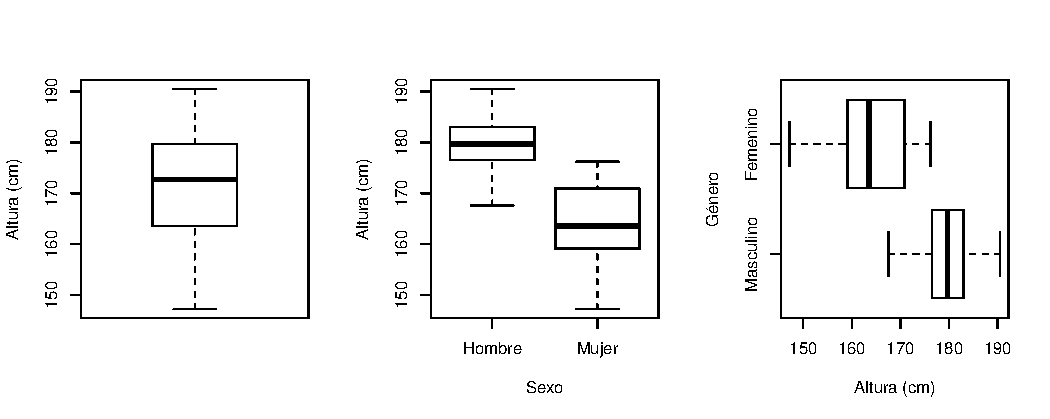
\includegraphics{Graficos_con_R_files/figure-latex/boxplots-1.pdf}
\caption{\label{fig:boxplots}Boxplot para la variable altura.}
\end{figure}

En la Figura \ref{fig:boxplots} se presentan los boxplots obtenidos con
las instrucciones anteriores. El segundo y tercer boxplot son el mismo,
lo único que se modificó fueron los nombres o etiquetas a colocar debajo
de cada boxplot por medio del argumento \texttt{names} y la orientación.

\section{\texorpdfstring{Función
\texttt{hist}}{Función hist}}\label{funcion-hist}

La función \texttt{hist} sirve para crear el histograma
\index{histograma}\index{hist} para una variable cuantitativa. Como
argumentos esta función recibe un vector con los datos y opcionalmente
puede ingresarse como argumento el número de intervalos a ser graficados
o en su defecto el número de clases se determina con la fórmula de
Sturges.

Nota: los programas de computador usualmente construyen los histogramas
automáticamente, sin embargo, un buen programa debe permitirnos elegir
el número de intervalos del histograma. Si usted posee un programa que
no le permite hacer cambios, cambie de programa.

La estructura de la función \texttt{hist} con los argumentos más comunes
de uso se muestran a continuación.

\begin{itemize}
\tightlist
\item
  \texttt{x}: vector numérico de valores para construir el histograma.
\item
  \texttt{breaks}: puede ser un número entero que indica el número
  aproximado de clases o un vector cuyos elementos indican los límites
  de los intervalos.
\item
  \texttt{freq}: argumento lógico; si se especifica como \texttt{TRUE},
  el histograma presentará frecuencias absolutas o conteo de datos para
  cada intervalo; si se especifica como \texttt{FALSE} el histograma
  presentar las frecuencias relativas (en porcentaje). Por defecto, este
  argumento toma el valor de \texttt{TRUE} siempre y cuando los
  intervalos sean de igual ancho.
\item
  \texttt{include.lowest}: argumento lógico; si se especifica como
  \texttt{TRUE}, un \texttt{x{[}i{]}} igual a los equal a un valor
  \texttt{breaks} se incluirá en la primera barra, si el argumento
  \texttt{right\ =\ TRUE}, o en la última en caso contrario.
\item
  \texttt{right}: argumento lógico; si es \texttt{TRUE}, los intervalos
  son abiertos a la izquierda y cerrados a la derecha \((a,b]\). Para la
  primera clase o intervalo si \texttt{include.lowest=TRUE} el valor más
  pequeño de los datos será incluido en éste. Si es \texttt{FALSE} los
  intervalos serán de la forma \([a,b)\) y el argumento
  \texttt{include.lowest=TRUE} tendrá el significado de incluir el ``más
  alto''.
\item
  \texttt{col}: para definir el color de las barras. Por defecto,
  \texttt{NULL} produce barras sin fondo.
\item
  \texttt{border}: para definir el color de los bordes de las barras.
\item
  \texttt{plot}: argumento lógico. Por defecto es \texttt{TRUE}, y el
  resultado es el gráfico del histograma; si se especifica como
  \texttt{FALSE} el resultado es una lista de conteos por cada
  intervalo.
\item
  \texttt{labels}: argumento lógico o carácter. Si se especifica como
  \texttt{TRUE} coloca etiquetas arriba de cada barra.
\item
  \texttt{...}: parámetros gráficos adicionales a \texttt{title} y
  \texttt{axis}.
\end{itemize}

\subsection*{Ejemplo}\label{ejemplo-2}


Vamos a construir varios histogramas para los tiempos de 180 corredores
de la media maratón de CONAVI realizada hace algunos años. A
continuación se muestra la forma de ingresar los 180 datos.

\begin{Shaded}
\begin{Highlighting}[]
\NormalTok{maraton <-}\StringTok{ }\KeywordTok{c}\NormalTok{(}
\DecValTok{10253}\NormalTok{, }\DecValTok{10302}\NormalTok{, }\DecValTok{10307}\NormalTok{, }\DecValTok{10309}\NormalTok{, }\DecValTok{10349}\NormalTok{, }\DecValTok{10353}\NormalTok{, }\DecValTok{10409}\NormalTok{, }\DecValTok{10442}\NormalTok{, }\DecValTok{10447}\NormalTok{, }
\DecValTok{10452}\NormalTok{, }\DecValTok{10504}\NormalTok{, }\DecValTok{10517}\NormalTok{, }\DecValTok{10530}\NormalTok{, }\DecValTok{10540}\NormalTok{, }\DecValTok{10549}\NormalTok{, }\DecValTok{10549}\NormalTok{, }\DecValTok{10606}\NormalTok{, }\DecValTok{10612}\NormalTok{, }
\DecValTok{10646}\NormalTok{, }\DecValTok{10648}\NormalTok{, }\DecValTok{10655}\NormalTok{, }\DecValTok{10707}\NormalTok{, }\DecValTok{10726}\NormalTok{, }\DecValTok{10731}\NormalTok{, }\DecValTok{10737}\NormalTok{, }\DecValTok{10743}\NormalTok{, }\DecValTok{10808}\NormalTok{, }
\DecValTok{10833}\NormalTok{, }\DecValTok{10843}\NormalTok{, }\DecValTok{10920}\NormalTok{, }\DecValTok{10938}\NormalTok{, }\DecValTok{10949}\NormalTok{, }\DecValTok{10954}\NormalTok{, }\DecValTok{10956}\NormalTok{, }\DecValTok{10958}\NormalTok{, }\DecValTok{11004}\NormalTok{, }
\DecValTok{11009}\NormalTok{, }\DecValTok{11024}\NormalTok{, }\DecValTok{11037}\NormalTok{, }\DecValTok{11045}\NormalTok{, }\DecValTok{11046}\NormalTok{, }\DecValTok{11049}\NormalTok{, }\DecValTok{11104}\NormalTok{, }\DecValTok{11127}\NormalTok{, }\DecValTok{11205}\NormalTok{, }
\DecValTok{11207}\NormalTok{, }\DecValTok{11215}\NormalTok{, }\DecValTok{11226}\NormalTok{, }\DecValTok{11233}\NormalTok{, }\DecValTok{11239}\NormalTok{, }\DecValTok{11307}\NormalTok{, }\DecValTok{11330}\NormalTok{, }\DecValTok{11342}\NormalTok{, }\DecValTok{11351}\NormalTok{, }
\DecValTok{11405}\NormalTok{, }\DecValTok{11413}\NormalTok{, }\DecValTok{11438}\NormalTok{, }\DecValTok{11453}\NormalTok{, }\DecValTok{11500}\NormalTok{, }\DecValTok{11501}\NormalTok{, }\DecValTok{11502}\NormalTok{, }\DecValTok{11503}\NormalTok{, }\DecValTok{11527}\NormalTok{, }
\DecValTok{11544}\NormalTok{, }\DecValTok{11549}\NormalTok{, }\DecValTok{11559}\NormalTok{, }\DecValTok{11612}\NormalTok{, }\DecValTok{11617}\NormalTok{, }\DecValTok{11635}\NormalTok{, }\DecValTok{11655}\NormalTok{, }\DecValTok{11731}\NormalTok{, }\DecValTok{11735}\NormalTok{,}
\DecValTok{11746}\NormalTok{, }\DecValTok{11800}\NormalTok{, }\DecValTok{11814}\NormalTok{, }\DecValTok{11828}\NormalTok{, }\DecValTok{11832}\NormalTok{, }\DecValTok{11841}\NormalTok{, }\DecValTok{11909}\NormalTok{, }\DecValTok{11926}\NormalTok{, }\DecValTok{11937}\NormalTok{, }
\DecValTok{11940}\NormalTok{, }\DecValTok{11947}\NormalTok{, }\DecValTok{11952}\NormalTok{, }\DecValTok{12005}\NormalTok{, }\DecValTok{12044}\NormalTok{, }\DecValTok{12113}\NormalTok{, }\DecValTok{12209}\NormalTok{, }\DecValTok{12230}\NormalTok{, }\DecValTok{12258}\NormalTok{, }
\DecValTok{12309}\NormalTok{, }\DecValTok{12327}\NormalTok{, }\DecValTok{12341}\NormalTok{, }\DecValTok{12413}\NormalTok{, }\DecValTok{12433}\NormalTok{, }\DecValTok{12440}\NormalTok{, }\DecValTok{12447}\NormalTok{, }\DecValTok{12530}\NormalTok{, }\DecValTok{12600}\NormalTok{, }
\DecValTok{12617}\NormalTok{, }\DecValTok{12640}\NormalTok{, }\DecValTok{12700}\NormalTok{, }\DecValTok{12706}\NormalTok{, }\DecValTok{12727}\NormalTok{, }\DecValTok{12840}\NormalTok{, }\DecValTok{12851}\NormalTok{, }\DecValTok{12851}\NormalTok{, }\DecValTok{12937}\NormalTok{,}
\DecValTok{13019}\NormalTok{, }\DecValTok{13040}\NormalTok{, }\DecValTok{13110}\NormalTok{, }\DecValTok{13114}\NormalTok{, }\DecValTok{13122}\NormalTok{, }\DecValTok{13155}\NormalTok{, }\DecValTok{13205}\NormalTok{, }\DecValTok{13210}\NormalTok{, }\DecValTok{13220}\NormalTok{, }
\DecValTok{13228}\NormalTok{, }\DecValTok{13307}\NormalTok{, }\DecValTok{13316}\NormalTok{, }\DecValTok{13335}\NormalTok{, }\DecValTok{13420}\NormalTok{, }\DecValTok{13425}\NormalTok{, }\DecValTok{13435}\NormalTok{, }\DecValTok{13435}\NormalTok{, }\DecValTok{13448}\NormalTok{, }
\DecValTok{13456}\NormalTok{, }\DecValTok{13536}\NormalTok{, }\DecValTok{13608}\NormalTok{, }\DecValTok{13612}\NormalTok{, }\DecValTok{13620}\NormalTok{, }\DecValTok{13646}\NormalTok{, }\DecValTok{13705}\NormalTok{, }\DecValTok{13730}\NormalTok{, }\DecValTok{13730}\NormalTok{, }
\DecValTok{13730}\NormalTok{, }\DecValTok{13747}\NormalTok{, }\DecValTok{13810}\NormalTok{, }\DecValTok{13850}\NormalTok{, }\DecValTok{13854}\NormalTok{, }\DecValTok{13901}\NormalTok{, }\DecValTok{13905}\NormalTok{, }\DecValTok{13907}\NormalTok{, }\DecValTok{13912}\NormalTok{,}
\DecValTok{13920}\NormalTok{, }\DecValTok{14000}\NormalTok{, }\DecValTok{14010}\NormalTok{, }\DecValTok{14025}\NormalTok{, }\DecValTok{14152}\NormalTok{, }\DecValTok{14208}\NormalTok{, }\DecValTok{14230}\NormalTok{, }\DecValTok{14344}\NormalTok{, }\DecValTok{14400}\NormalTok{, }
\DecValTok{14455}\NormalTok{, }\DecValTok{14509}\NormalTok{, }\DecValTok{14552}\NormalTok{, }\DecValTok{14652}\NormalTok{, }\DecValTok{15009}\NormalTok{, }\DecValTok{15026}\NormalTok{, }\DecValTok{15242}\NormalTok{, }\DecValTok{15406}\NormalTok{, }\DecValTok{15409}\NormalTok{, }
\DecValTok{15528}\NormalTok{, }\DecValTok{15549}\NormalTok{, }\DecValTok{15644}\NormalTok{, }\DecValTok{15758}\NormalTok{, }\DecValTok{15837}\NormalTok{, }\DecValTok{15916}\NormalTok{, }\DecValTok{15926}\NormalTok{, }\DecValTok{15948}\NormalTok{, }\DecValTok{20055}\NormalTok{, }
\DecValTok{20416}\NormalTok{, }\DecValTok{20520}\NormalTok{, }\DecValTok{20600}\NormalTok{, }\DecValTok{20732}\NormalTok{, }\DecValTok{20748}\NormalTok{, }\DecValTok{20916}\NormalTok{, }\DecValTok{21149}\NormalTok{, }\DecValTok{21714}\NormalTok{, }\DecValTok{23256}\NormalTok{)}
\end{Highlighting}
\end{Shaded}

Los datos están codificados como por seis números en el formato hmmss,
donde h corresponde a las horas, mm a los minutos y ss a los segundos
necesarios para completar la maratón. Antes de construir los histogramas
es necesario convertir los tiempos anteriores almacenados en
\texttt{maraton} a horas, para esto se utiliza el siguiente código.

\begin{Shaded}
\begin{Highlighting}[]
\NormalTok{horas <-}\StringTok{ }\NormalTok{maraton %/%}\StringTok{ }\DecValTok{10000}
\NormalTok{min <-}\StringTok{ }\NormalTok{(maraton -}\StringTok{ }\NormalTok{horas *}\StringTok{ }\DecValTok{10000}\NormalTok{) %/%}\StringTok{ }\DecValTok{100}
\NormalTok{seg <-}\StringTok{ }\NormalTok{maraton -}\StringTok{ }\NormalTok{horas *}\StringTok{ }\DecValTok{10000} \NormalTok{-}\StringTok{ }\NormalTok{min *}\StringTok{ }\DecValTok{100}
\NormalTok{Tiempos <-}\StringTok{ }\NormalTok{horas +}\StringTok{ }\NormalTok{min /}\StringTok{ }\DecValTok{60} \NormalTok{+}\StringTok{ }\NormalTok{seg /}\StringTok{ }\DecValTok{3600}
\end{Highlighting}
\end{Shaded}

A continuación se muestra el código para construir cuatro histogramas
con 2, 4, 8 y 16 intervalos para los tiempos a partir de la variable
\texttt{Tiempos}.

\begin{Shaded}
\begin{Highlighting}[]
\KeywordTok{par}\NormalTok{(}\DataTypeTok{mfrow=}\KeywordTok{c}\NormalTok{(}\DecValTok{2}\NormalTok{,}\DecValTok{2}\NormalTok{))}

\KeywordTok{hist}\NormalTok{(}\DataTypeTok{x=}\NormalTok{Tiempos, }\DataTypeTok{breaks=}\DecValTok{2}\NormalTok{, }\DataTypeTok{main=}\StringTok{""}\NormalTok{, }\DataTypeTok{xlab=}\StringTok{"Tiempo (horas)"}\NormalTok{,}
     \DataTypeTok{ylab=}\StringTok{"Frecuencias"}\NormalTok{, }\DataTypeTok{las=}\DecValTok{1}\NormalTok{)}
\KeywordTok{mtext}\NormalTok{(}\StringTok{"(A)"}\NormalTok{, }\DataTypeTok{side=}\DecValTok{1}\NormalTok{, }\DataTypeTok{line=}\DecValTok{4}\NormalTok{, }\DataTypeTok{font=}\DecValTok{1}\NormalTok{)}

\KeywordTok{hist}\NormalTok{(}\DataTypeTok{x=}\NormalTok{Tiempos, }\DataTypeTok{breaks=}\DecValTok{4}\NormalTok{, }\DataTypeTok{main=}\StringTok{""}\NormalTok{, }\DataTypeTok{xlab=}\StringTok{"Tiempo (horas)"}\NormalTok{,}
     \DataTypeTok{ylab=}\StringTok{"Frecuencias"}\NormalTok{, }\DataTypeTok{las=}\DecValTok{1}\NormalTok{)}
\KeywordTok{mtext}\NormalTok{(}\StringTok{"(B)"}\NormalTok{, }\DataTypeTok{side=}\DecValTok{1}\NormalTok{, }\DataTypeTok{line=}\DecValTok{4}\NormalTok{, }\DataTypeTok{font=}\DecValTok{1}\NormalTok{)}

\KeywordTok{hist}\NormalTok{(}\DataTypeTok{x=}\NormalTok{Tiempos, }\DataTypeTok{breaks=}\DecValTok{8}\NormalTok{, }\DataTypeTok{main=}\StringTok{""}\NormalTok{, }\DataTypeTok{xlab=}\StringTok{"Tiempo (horas)"}\NormalTok{,}
     \DataTypeTok{ylab=}\StringTok{"Frecuencias"}\NormalTok{)}
\KeywordTok{mtext}\NormalTok{(}\StringTok{"(C)"}\NormalTok{, }\DataTypeTok{side=}\DecValTok{1}\NormalTok{, }\DataTypeTok{line=}\DecValTok{4}\NormalTok{, }\DataTypeTok{font=}\DecValTok{1}\NormalTok{)}

\KeywordTok{hist}\NormalTok{(}\DataTypeTok{x=}\NormalTok{Tiempos, }\DataTypeTok{breaks=}\DecValTok{16}\NormalTok{, }\DataTypeTok{main=}\StringTok{""}\NormalTok{, }\DataTypeTok{xlab=}\StringTok{"Tiempo (horas)"}\NormalTok{,}
     \DataTypeTok{ylab=}\StringTok{"Frecuencias"}\NormalTok{)}
\KeywordTok{mtext}\NormalTok{(}\StringTok{"(D)"}\NormalTok{, }\DataTypeTok{side=}\DecValTok{1}\NormalTok{, }\DataTypeTok{line=}\DecValTok{4}\NormalTok{, }\DataTypeTok{font=}\DecValTok{1}\NormalTok{)}
\end{Highlighting}
\end{Shaded}

\begin{figure}[htbp]
\centering
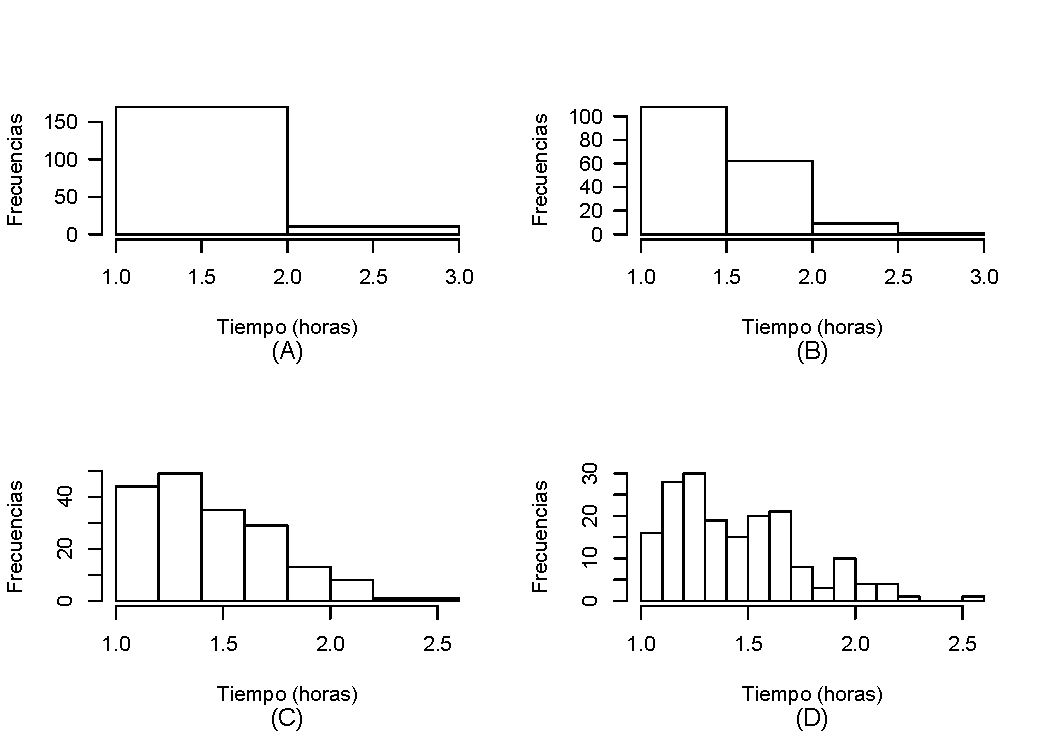
\includegraphics{Graficos_con_R_files/figure-latex/hist1-1.pdf}
\caption{\label{fig:hist1}Histogramas para el tiempo en la media maratón de
CONAVI. A: histograma con dos intervalos, B: histograma con cuatro
intervalos, C: histograma con seis intervalos, C: histograma con 18
intervalos.}
\end{figure}

En la Figura \ref{fig:hist1} se presentan los cuatro histogramas. El
histograma C, con 8 barras, muestra más claramente la asimetría (este es
el que la mayoría de los programas produce por defecto, ya que la regla
de Sturges para este conjunto de datos aproxima a 8 barras). Si
consideramos más barras por ejemplo 16, como tenemos en D, se refina más
la información y empezamos a notar multimodalidad. En el código anterior
se incluyó \texttt{las\ =\ 1} para conseguir que los número del eje Y
queden escritos de forma horizontal, ver A y B en Figura
\ref{fig:hist1}.

A continuación vamos a construir cuatro histogramas: el primero con dos
intervalos intervalos y puntos de corte dados por el mínimo, la mediana
y el máximo; el segundo con tres intervalos y puntos de corte dados por
el mínimo, cuartiles 1, 2, 3 y máximo; el cuarto con diez intervalos y
puntos de corte dados por los deciles; y el último con veinte intervalos
y puntos de corte dados por cuantiles 5, 10, \(\ldots\), 95. En el
código mostrado a continuación se presenta la creación de los puntos de
corte y los cuatro histogramas.

\begin{Shaded}
\begin{Highlighting}[]
\NormalTok{puntos1 <-}\StringTok{ }\KeywordTok{c}\NormalTok{(}\KeywordTok{quantile}\NormalTok{(Tiempos, }\DataTypeTok{probs=}\KeywordTok{c}\NormalTok{(}\DecValTok{0}\NormalTok{, }\FloatTok{0.5}\NormalTok{, }\DecValTok{1}\NormalTok{)))}
\NormalTok{puntos2 <-}\StringTok{ }\KeywordTok{c}\NormalTok{(}\KeywordTok{quantile}\NormalTok{(Tiempos, }\DataTypeTok{probs=}\KeywordTok{c}\NormalTok{(}\DecValTok{0}\NormalTok{, }\FloatTok{0.25}\NormalTok{, }\FloatTok{0.5}\NormalTok{, }\FloatTok{0.75}\NormalTok{, }\DecValTok{1}\NormalTok{)))}
\NormalTok{puntos3 <-}\StringTok{ }\KeywordTok{c}\NormalTok{(}\KeywordTok{quantile}\NormalTok{(Tiempos, }\DataTypeTok{probs=}\KeywordTok{seq}\NormalTok{(}\DecValTok{0}\NormalTok{, }\DecValTok{1}\NormalTok{, }\DataTypeTok{by=}\FloatTok{0.1}\NormalTok{)))}
\NormalTok{puntos4 <-}\StringTok{ }\KeywordTok{c}\NormalTok{(}\KeywordTok{quantile}\NormalTok{(Tiempos, }\DataTypeTok{probs=}\KeywordTok{seq}\NormalTok{(}\DecValTok{0}\NormalTok{, }\DecValTok{1}\NormalTok{, }\DataTypeTok{by=}\FloatTok{0.05}\NormalTok{)))}

\KeywordTok{par}\NormalTok{(}\DataTypeTok{mfrow=}\KeywordTok{c}\NormalTok{(}\DecValTok{2}\NormalTok{, }\DecValTok{2}\NormalTok{))}
\KeywordTok{hist}\NormalTok{(Tiempos, }\DataTypeTok{breaks=}\NormalTok{puntos1, }\DataTypeTok{freq=}\OtherTok{FALSE}\NormalTok{, }\DataTypeTok{ylim=}\KeywordTok{c}\NormalTok{(}\DecValTok{0}\NormalTok{,}\DecValTok{2}\NormalTok{), }\DataTypeTok{labels=}\OtherTok{TRUE}\NormalTok{,}
     \DataTypeTok{main=}\StringTok{""}\NormalTok{, }\DataTypeTok{ylab=}\StringTok{"Densidad"}\NormalTok{)}
\KeywordTok{mtext}\NormalTok{(}\StringTok{"(A)"}\NormalTok{, }\DataTypeTok{side=}\DecValTok{1}\NormalTok{, }\DataTypeTok{line=}\DecValTok{4}\NormalTok{, }\DataTypeTok{font=}\DecValTok{1}\NormalTok{)}
\KeywordTok{hist}\NormalTok{(Tiempos, }\DataTypeTok{breaks=}\NormalTok{puntos2, }\DataTypeTok{freq=}\OtherTok{FALSE}\NormalTok{, }\DataTypeTok{ylim=}\KeywordTok{c}\NormalTok{(}\DecValTok{0}\NormalTok{,}\DecValTok{2}\NormalTok{), }\DataTypeTok{labels=}\OtherTok{TRUE}\NormalTok{,}
     \DataTypeTok{main=}\StringTok{""}\NormalTok{, }\DataTypeTok{ylab=}\StringTok{"Densidad"}\NormalTok{)}
\KeywordTok{mtext}\NormalTok{(}\StringTok{"(B)"}\NormalTok{, }\DataTypeTok{side=}\DecValTok{1}\NormalTok{, }\DataTypeTok{line=}\DecValTok{4}\NormalTok{, }\DataTypeTok{font=}\DecValTok{1}\NormalTok{)}
\KeywordTok{hist}\NormalTok{(Tiempos, }\DataTypeTok{breaks=}\NormalTok{puntos3, }\DataTypeTok{freq=}\OtherTok{FALSE}\NormalTok{, }\DataTypeTok{ylim=}\KeywordTok{c}\NormalTok{(}\DecValTok{0}\NormalTok{,}\DecValTok{2}\NormalTok{),}
     \DataTypeTok{main=}\StringTok{""}\NormalTok{, }\DataTypeTok{ylab=}\StringTok{"Densidad"}\NormalTok{)}
\KeywordTok{mtext}\NormalTok{(}\StringTok{"(C)"}\NormalTok{, }\DataTypeTok{side=}\DecValTok{1}\NormalTok{, }\DataTypeTok{line=}\DecValTok{4}\NormalTok{, }\DataTypeTok{font=}\DecValTok{1}\NormalTok{)}
\KeywordTok{hist}\NormalTok{(Tiempos, }\DataTypeTok{breaks=}\NormalTok{puntos4, }\DataTypeTok{freq=}\OtherTok{FALSE}\NormalTok{, }\DataTypeTok{ylim=}\KeywordTok{c}\NormalTok{(}\DecValTok{0}\NormalTok{,}\DecValTok{2}\NormalTok{),}
     \DataTypeTok{main=}\StringTok{""}\NormalTok{, }\DataTypeTok{ylab=}\StringTok{"Densidad"}\NormalTok{)}
\KeywordTok{mtext}\NormalTok{(}\StringTok{"(D)"}\NormalTok{, }\DataTypeTok{side=}\DecValTok{1}\NormalTok{, }\DataTypeTok{line=}\DecValTok{4}\NormalTok{, }\DataTypeTok{font=}\DecValTok{1}\NormalTok{)}
\end{Highlighting}
\end{Shaded}

\begin{figure}[htbp]
\centering
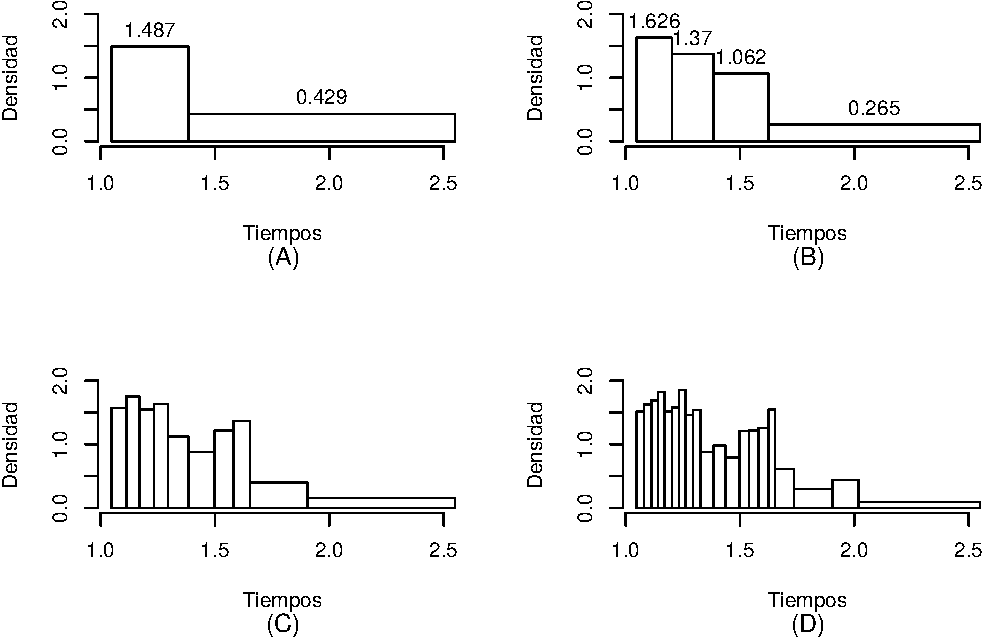
\includegraphics{Graficos_con_R_files/figure-latex/hist2-1.pdf}
\caption{\label{fig:hist2}Histogramas para el tiempo en la media maratón de
CONAVI. A: histograma con dos intervalos, B: histograma con cuatro
intervalos, C: histograma con diez intervalos, C: histograma con veinte
intervalos.}
\end{figure}

Nota: En estos histogramas, las alturas corresponden a las intensidades
(frec. relativa/long. intervalo). Por tanto, el área de cada rectángulo
da cuenta de las frecuencias relativas. Para el caso (A) ambos
intervalos tienen igual área y cada uno contiene 50\% de los datos. esto
puede verificarse así:

\begin{verbatim}
Intensidad primera clase = 1.4869888 = 0.5 / (1.384306 - 1.048056)
Intensidad segunda clase = 0.4293381 = 0.5 / (2.548889 - 1.384306)
\end{verbatim}

\section{\texorpdfstring{Función \texttt{qqnorm} y \texttt{qqplot}
\index{qqnorm}
\index{qqplot}}{Función qqnorm y qqplot  }}\label{funcion-qqnorm-y-qqplot}

Los gráficos cuantil cuantil (quantile-quantile plot) son una ayuda para
explorar si un conjunto de datos o muestra proviene de una población con
cierta distribución.

La función \texttt{qqnorm} sirve para explorar la normalidad de una
muestra mientras que la función \texttt{qqplot} es de propósito más
general, sirve para crear el gráfico cuantil cuantil para cualquier
distribución.

La estructura de las funciones con los argumentos más comunes de uso se
muestran a continuación.

\begin{Shaded}
\begin{Highlighting}[]
\KeywordTok{qqnorm}\NormalTok{(y, ...)}
\KeywordTok{qqplot}\NormalTok{(y, x, ...)}
\end{Highlighting}
\end{Shaded}

La función \texttt{qqnorm} sólo necesita que se le ingrese el vector con
la muestra por medio del parámetro \texttt{y}, la función
\texttt{qqplot} necesita de la muestra en el parámetro \texttt{y} y que
se ingrese en el parámetro \texttt{x} los cuantiles de la población
candidata.

Existe otra función útil y es \texttt{qqline}, esta función sirve para
agregar una línea de referencia al gráfico cuantil cuantil obtenido con
\texttt{qqnorm}.

\subsection*{Ejemplo}\label{ejemplo-3}


Simular 30 observaciones de una distribución \(N(\mu=10, \sigma=4)\) y
construir el gráfico cuantil cuantil.

El código para simular la muestra y crear el gráfico cuantil cuantil se
muestra a continuación.

\begin{Shaded}
\begin{Highlighting}[]
\NormalTok{muestra <-}\StringTok{ }\KeywordTok{rnorm}\NormalTok{(}\DataTypeTok{n=}\DecValTok{30}\NormalTok{, }\DataTypeTok{mean=}\DecValTok{10}\NormalTok{, }\DataTypeTok{sd=}\DecValTok{4}\NormalTok{)}

\KeywordTok{par}\NormalTok{(}\DataTypeTok{mfrow=}\KeywordTok{c}\NormalTok{(}\DecValTok{1}\NormalTok{, }\DecValTok{2}\NormalTok{))}

\KeywordTok{qqnorm}\NormalTok{(}\DataTypeTok{y=}\NormalTok{muestra)}
\KeywordTok{qqline}\NormalTok{(}\DataTypeTok{y=}\NormalTok{muestra)}

\KeywordTok{qqnorm}\NormalTok{(}\DataTypeTok{y=}\NormalTok{muestra, }\DataTypeTok{main=}\StringTok{''}\NormalTok{, }\DataTypeTok{ylab=}\StringTok{'Cuantiles muestrales'}\NormalTok{,}
       \DataTypeTok{xlab=}\StringTok{'Cuantiles teóricos'}\NormalTok{, }\DataTypeTok{las=}\DecValTok{1}\NormalTok{)}
\KeywordTok{qqline}\NormalTok{(}\DataTypeTok{y=}\NormalTok{muestra, }\DataTypeTok{col=}\StringTok{'blue'}\NormalTok{, }\DataTypeTok{lwd=}\DecValTok{2}\NormalTok{, }\DataTypeTok{lty=}\DecValTok{2}\NormalTok{)}
\end{Highlighting}
\end{Shaded}

\begin{figure}[htbp]
\centering
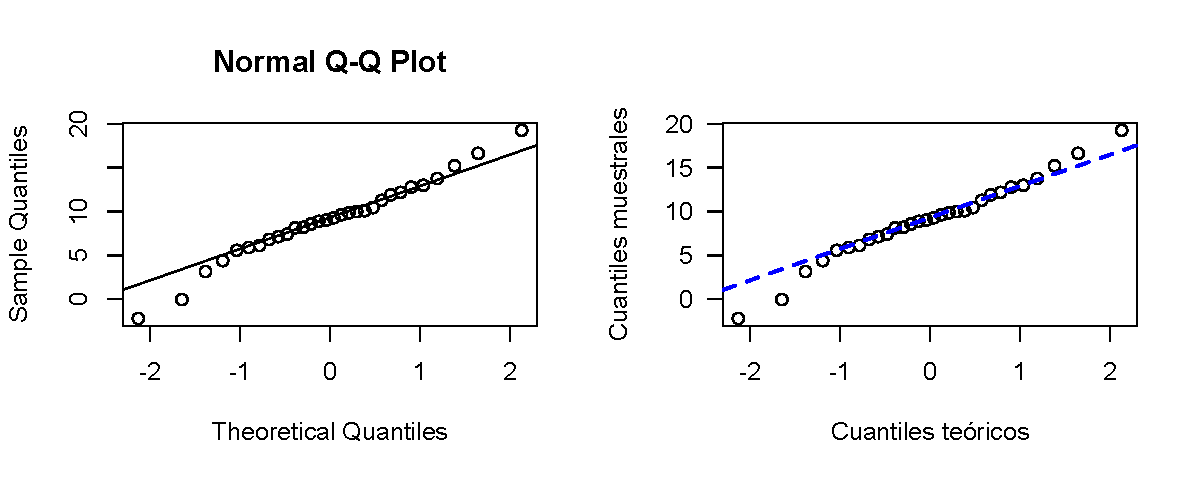
\includegraphics{Graficos_con_R_files/figure-latex/qqplot1-1.pdf}
\caption{\label{fig:qqplot1}Gráfico cuantil cuantil para una muestra
generada de una población normal.}
\end{figure}

En la izquierda de la Figura \ref{fig:qqplot1} está el gráfico cuantil
cuantil sin editar, en la derecha se encuentra el gráfico luego de
modificar los nombres de los ejes, grosor y color de la línea de
referencia.

\subsection*{Ejemplo}\label{ejemplo-4}


Simular 100 observaciones de una distribución \(Weibull(1,1)\) y
construir dos gráficos cuantil cuantil, el primero tomando como
referencia los cuantiles de una \(N(0,1)\) y el segundo tomando los
cuantiles de la \(Weibull(1,1)\).

El código para simular la muestra y crear los gráficos cuantil cuantil
se muestra a continuación.

\begin{Shaded}
\begin{Highlighting}[]
\NormalTok{n <-}\StringTok{ }\DecValTok{100}
\NormalTok{muestra <-}\StringTok{ }\KeywordTok{rweibull}\NormalTok{(}\DataTypeTok{n=}\NormalTok{n, }\DataTypeTok{shape=}\DecValTok{1}\NormalTok{, }\DataTypeTok{scale=}\DecValTok{1}\NormalTok{)}

\KeywordTok{par}\NormalTok{(}\DataTypeTok{mfrow=}\KeywordTok{c}\NormalTok{(}\DecValTok{1}\NormalTok{, }\DecValTok{2}\NormalTok{))}
\KeywordTok{qqplot}\NormalTok{(}\DataTypeTok{y=}\NormalTok{muestra, }\DataTypeTok{x=}\KeywordTok{qnorm}\NormalTok{(}\KeywordTok{ppoints}\NormalTok{(n)))}
\KeywordTok{qqplot}\NormalTok{(}\DataTypeTok{y=}\NormalTok{muestra, }\DataTypeTok{x=}\KeywordTok{qweibull}\NormalTok{(}\KeywordTok{ppoints}\NormalTok{(n), }\DataTypeTok{shape=}\DecValTok{1}\NormalTok{, }\DataTypeTok{scale=}\DecValTok{1}\NormalTok{))}
\end{Highlighting}
\end{Shaded}

\begin{figure}[htbp]
\centering
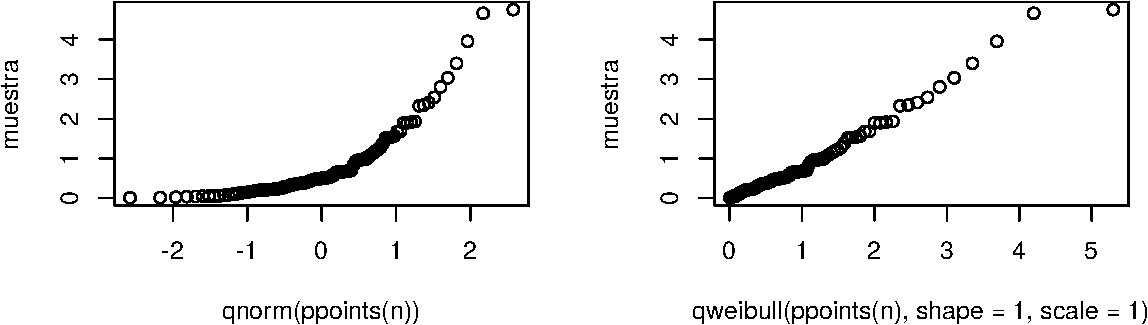
\includegraphics{Graficos_con_R_files/figure-latex/qqplot2-1.pdf}
\caption{\label{fig:qqplot2}Gráfico cuantil cuantil para una muestra
generada de una población Weibull.}
\end{figure}

En la Figura \ref{fig:qqplot2} están los gráficos cuantil cuantil
solicitados. Del pánel izquierdo de la figura vemos que los puntos NO
están alineados, esto indica que la muestra no proviene de la
distribución \(N(0, 1)\), esto es un resultado esperado ya que sabíamos
que la muestra no fue generada de una normal. En el pánel derecho de la
misma figura vemos que los puntos SI están alineados, esto indica que la
muestra generada puede provenir de una población \(Weibull(1, 1)\). Los
nombres de los ejes en la Figura \ref{fig:qqplot2} pueden ser editados
para presentar una figura con mejor apariencia.

\section{\texorpdfstring{Función \texttt{density} \index{density}
\index{densidad}}{Función density  }}\label{funcion-density}

Los gráficos de densidad son muy útiles porque permiten ver el(los)
intervalo(s) donde una variable cuantitativa puede ocurrir con mayor
probabilidad.

La función \texttt{density} crea la información de la densidad y la
función \texttt{plot} dibuja la densidad.

La estructura de la función \texttt{density} con los argumentos más
comunes de uso se muestra a continuación.

\begin{Shaded}
\begin{Highlighting}[]
\KeywordTok{density}\NormalTok{(x, bw, }\DataTypeTok{adjust=}\DecValTok{1}\NormalTok{, }\DataTypeTok{kernel=}\StringTok{'gaussian'}\NormalTok{, }\DataTypeTok{na.rm=}\OtherTok{FALSE}\NormalTok{)}
\end{Highlighting}
\end{Shaded}

Los argumentos de la función \texttt{density} son:

\begin{itemize}
\tightlist
\item
  \texttt{x}: vector con los datos para los cuales se quiere la
  densidad.
\item
  \texttt{bw}: ancho de banda.
\item
  \texttt{kernel}: núcleo de suavización a usar, los posibles valores
  son \texttt{gaussian}, \texttt{rectangular}, \texttt{triangular},
  \texttt{epanechnikov}, \texttt{biweight}, \texttt{cosine} o
  \texttt{optcosine}, el valor por defecto es \texttt{gaussian}.
\item
  \texttt{na.rm}: valor lógico, si es \texttt{TRUE} se eliminan los
  valores con \texttt{NA} para construir la densidad, el valor por
  defecto es \texttt{FALSE}.
\end{itemize}

\subsection*{Ejemplo}\label{ejemplo-5}


Simular mil observaciones de una \(N(0, 1)\), aplicar la función
\texttt{density} al vector y explorar el contenido de la salida.

Primero se generan las observaciones y se almacenan en el objeto
\texttt{y}, luego se aplica la función \texttt{density} y el resultado
se guarda en el objeto \texttt{res}, para explorar lo que almacena
\texttt{res} se usa la función \texttt{names}. A continuación el código
utilizado.

\begin{Shaded}
\begin{Highlighting}[]
\NormalTok{y <-}\StringTok{ }\KeywordTok{rnorm}\NormalTok{(}\DataTypeTok{n=}\DecValTok{1000}\NormalTok{)}
\NormalTok{res <-}\StringTok{ }\KeywordTok{density}\NormalTok{(y)}
\KeywordTok{names}\NormalTok{(res)}
\end{Highlighting}
\end{Shaded}

\begin{verbatim}
## [1] "x"         "y"         "bw"        "n"        
## [5] "call"      "data.name" "has.na"
\end{verbatim}

De la salida anterior se observa que la lista \texttt{res} tiene 7
elementos, los dos primeros son los vectores con las coordenadas para
dibujar la densidad, los restantes elementos con información adicional.

\subsection*{Ejemplo}\label{ejemplo-6}


Con los datos generados en el ejemplo anterior construir la densidad
para varios núcleo y para varios valores de ancho de banda.

En el siguiente código se construyen 4 densidades para diferentes
núcleos.

\begin{Shaded}
\begin{Highlighting}[]
\KeywordTok{par}\NormalTok{(}\DataTypeTok{mfrow=}\KeywordTok{c}\NormalTok{(}\DecValTok{2}\NormalTok{, }\DecValTok{2}\NormalTok{))}
\KeywordTok{plot}\NormalTok{(}\KeywordTok{density}\NormalTok{(y, }\DataTypeTok{kernel=}\StringTok{'gaussian'}\NormalTok{))}
\KeywordTok{plot}\NormalTok{(}\KeywordTok{density}\NormalTok{(y, }\DataTypeTok{kernel=}\StringTok{'triangular'}\NormalTok{))}
\KeywordTok{plot}\NormalTok{(}\KeywordTok{density}\NormalTok{(y, }\DataTypeTok{kernel=}\StringTok{'cosine'}\NormalTok{))}
\KeywordTok{plot}\NormalTok{(}\KeywordTok{density}\NormalTok{(y, }\DataTypeTok{kernel=}\StringTok{'rectangular'}\NormalTok{))}
\end{Highlighting}
\end{Shaded}

\begin{figure}[htbp]
\centering
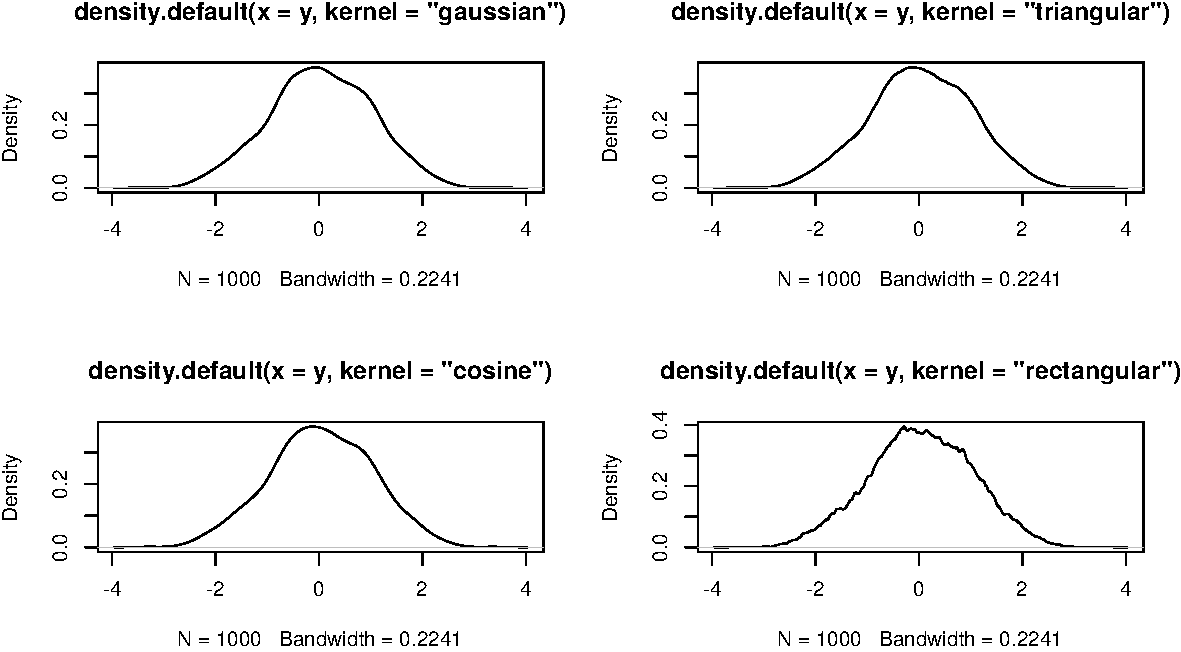
\includegraphics{Graficos_con_R_files/figure-latex/density1-1.pdf}
\caption{\label{fig:density1}Densidad para una muestra aleatoria de una N(0,
1) cambiando el núcleo de la densidad.}
\end{figure}

En la Figura \ref{fig:density1} se muestran las densidades para 4
elecciones del núcleo. En la práctica se usa el núcleo que está por
defecto (\texttt{gaussian}) ya que el objetivo de una densidad es ver la
zonas donde es más probable encontrar observaciones de la variable.

En el siguiente código se construyen 4 densidades para diferentes anchos
de banda.

\begin{Shaded}
\begin{Highlighting}[]
\KeywordTok{par}\NormalTok{(}\DataTypeTok{mfrow=}\KeywordTok{c}\NormalTok{(}\DecValTok{2}\NormalTok{, }\DecValTok{2}\NormalTok{))}
\KeywordTok{plot}\NormalTok{(}\KeywordTok{density}\NormalTok{(y, }\DataTypeTok{bw=}\FloatTok{0.1}\NormalTok{))}
\KeywordTok{plot}\NormalTok{(}\KeywordTok{density}\NormalTok{(y, }\DataTypeTok{bw=}\FloatTok{0.2241}\NormalTok{))  }\CommentTok{# bw obtenido antes}
\KeywordTok{plot}\NormalTok{(}\KeywordTok{density}\NormalTok{(y, }\DataTypeTok{bw=}\FloatTok{0.5}\NormalTok{))}
\KeywordTok{plot}\NormalTok{(}\KeywordTok{density}\NormalTok{(y, }\DataTypeTok{bw=}\DecValTok{1}\NormalTok{))}
\end{Highlighting}
\end{Shaded}

\begin{figure}[htbp]
\centering
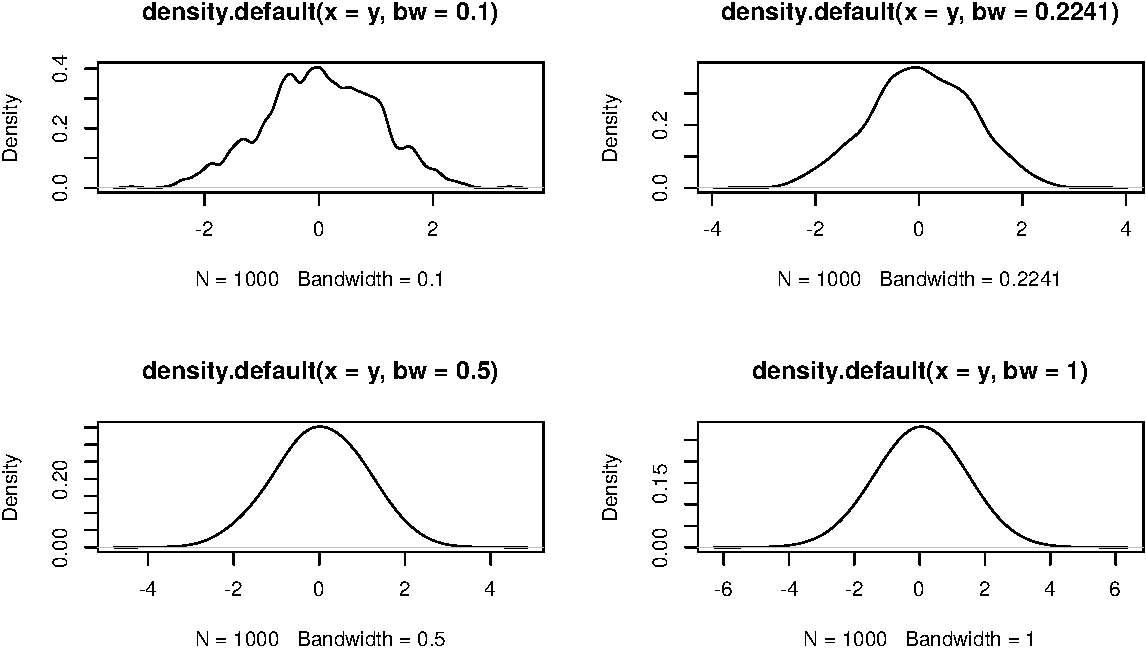
\includegraphics{Graficos_con_R_files/figure-latex/density2-1.pdf}
\caption{\label{fig:density2}Densidad para una muestra aleatoria de una N(0,
1) cambiando el ancho de banda.}
\end{figure}

En la Figura \ref{fig:density2} se muestran las densidades para 4
elecciones del parámetro ancho de banda \texttt{bw}, el valor de 0.2241
fue el valor calculado automáticamente por \proglang{R} y fue obtenido
de la Figura \ref{fig:density1}, los otros valores fueron elegidos
arbitrariamente para ver los cambios en la densidad. El usar un ancho de
banda pequeño la densidad queda muy rugosa y usar un valor muy grande la
suaviza, se recomienda usar el valor automático.

\subsection*{Ejemplo}\label{ejemplo-7}


Construir un gráfico de densidad para la variable peso corporal de la
base de datos \texttt{medidas\_cuerpo}, luego construir la densidad para
la misma variable pero diferenciando por sexo.

\begin{Shaded}
\begin{Highlighting}[]
\NormalTok{url <-}\StringTok{ 'https://raw.githubusercontent.com/fhernanb/datos/master/medidas_cuerpo'}
\NormalTok{datos <-}\StringTok{ }\KeywordTok{read.table}\NormalTok{(}\DataTypeTok{file=}\NormalTok{url, }\DataTypeTok{header=}\NormalTok{T)}

\KeywordTok{par}\NormalTok{(}\DataTypeTok{mfrow=}\KeywordTok{c}\NormalTok{(}\DecValTok{1}\NormalTok{, }\DecValTok{2}\NormalTok{))}
\KeywordTok{plot}\NormalTok{(}\KeywordTok{density}\NormalTok{(datos$peso), }\DataTypeTok{main=}\StringTok{'Densidad para el peso corporal'}\NormalTok{,}
     \DataTypeTok{xlab=}\StringTok{'Peso corporal (kg)'}\NormalTok{, }\DataTypeTok{ylab=}\StringTok{'Densidad'}\NormalTok{, }\DataTypeTok{lwd=}\DecValTok{4}\NormalTok{)}

\NormalTok{den.hom <-}\StringTok{ }\KeywordTok{with}\NormalTok{(datos, }\KeywordTok{density}\NormalTok{(peso[sexo ==}\StringTok{ 'Hombre'}\NormalTok{]))}
\NormalTok{den.muj <-}\StringTok{ }\KeywordTok{with}\NormalTok{(datos, }\KeywordTok{density}\NormalTok{(peso[sexo ==}\StringTok{ 'Mujer'}\NormalTok{]))}

\KeywordTok{plot}\NormalTok{(den.hom, }\DataTypeTok{xlim=}\KeywordTok{c}\NormalTok{(}\DecValTok{20}\NormalTok{, }\DecValTok{120}\NormalTok{), }
     \DataTypeTok{main=}\StringTok{'Densidad para el peso corporal'}\NormalTok{, }\DataTypeTok{ylab=}\StringTok{'Densidad'}\NormalTok{,}
     \DataTypeTok{xlab=}\StringTok{'Peso corporal (kg)'}\NormalTok{, }\DataTypeTok{lwd=}\DecValTok{4}\NormalTok{, }\DataTypeTok{col=}\StringTok{'blue'}\NormalTok{)}
\KeywordTok{lines}\NormalTok{(den.muj, }\DataTypeTok{lwd=}\DecValTok{4}\NormalTok{, }\DataTypeTok{col=}\StringTok{'red'}\NormalTok{)}
\KeywordTok{legend}\NormalTok{(}\StringTok{'topright'}\NormalTok{, }\DataTypeTok{legend=}\KeywordTok{c}\NormalTok{(}\StringTok{'Hombres'}\NormalTok{, }\StringTok{'Mujeres'}\NormalTok{), }\DataTypeTok{bty=}\StringTok{'n'}\NormalTok{,}
       \DataTypeTok{lwd=}\DecValTok{3}\NormalTok{, }\DataTypeTok{col=}\KeywordTok{c}\NormalTok{(}\StringTok{'blue'}\NormalTok{, }\StringTok{'red'}\NormalTok{))}
\end{Highlighting}
\end{Shaded}

\begin{figure}[htbp]
\centering
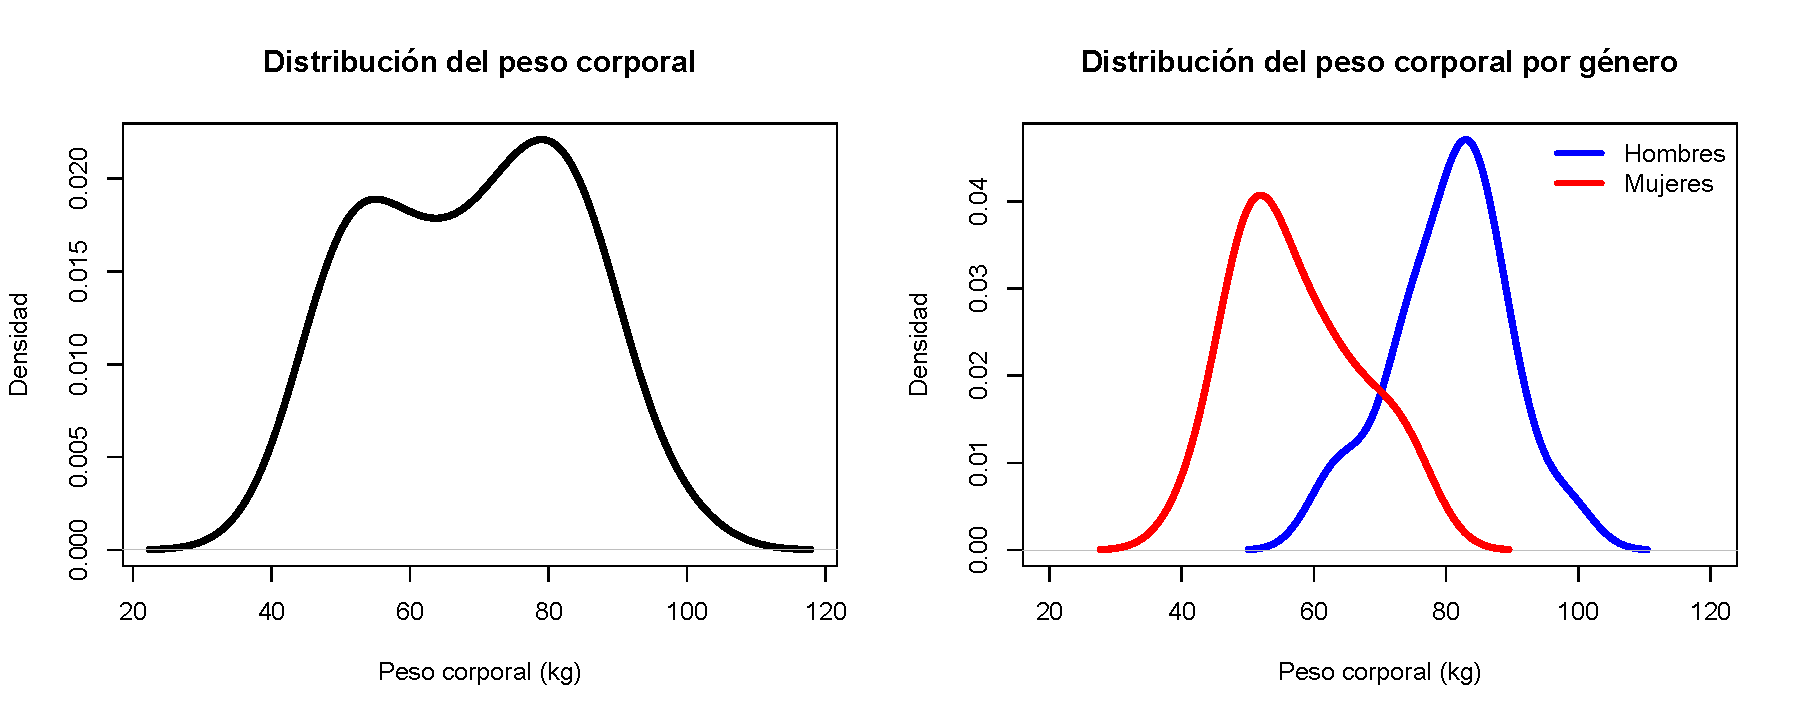
\includegraphics{Graficos_con_R_files/figure-latex/density3-1.pdf}
\caption{\label{fig:density3}Densidad para la variable peso en la izquierda,
densidad para el peso diferenciando por sexo a la derecha.}
\end{figure}

En el panel izquierdo de la Figura \ref{fig:density3} se muestra la
densidad para la variable peso, de esta figura se observa que tiene dos
sectores de mayor densidad, alrededor de 50 kg y alrededor de 80 kg. En
el panel izquierdo están la densidades del peso corporal para hombres y
mujeres, aquí se observa claramente la diferencia entre los pesos de
hombres y mujeres.

\chapter{Gráficos para una variable
cualitativa}\label{graficos-para-una-variable-cualitativa}

En este capítulo se presentan funciones para la creación de gráficos con
una sola variable cualitativa.

\section{\texorpdfstring{Función \texttt{barplot}
\index{gráfico de barras}
\index{barplot}}{Función barplot  }}\label{funcion-barplot}

Los gráficos de barras son útiles para representar las frecuencias
absolutas o relativas asociadas a los niveles de una variable
cualitativa.

La función \texttt{barplot} se usa para obtener un gráfico de barras. La
estructura de la función \texttt{barplot} con los argumentos más comunes
de uso se muestra a continuación.

\begin{Shaded}
\begin{Highlighting}[]
\KeywordTok{barplot}\NormalTok{(height, )}
\end{Highlighting}
\end{Shaded}

Los argumentos de la función \texttt{barplot} son:

\begin{itemize}
\tightlist
\item
  \texttt{height}: vector o matriz con la información de las frecuencias
  absolutas o relativas.
\end{itemize}

\subsection*{Ejemplo}\label{ejemplo-8}


Suponga que queremos construir un diagrama de barras para las
frecuencias relativas para la variable estrato socioeconómico del
apartamento de la base de datos sobre apartamentos usados en Medellín.

A continuación se muestra el código necesario para cargar la base de
datos \texttt{aptos2015}. Antes de construir el diagrama de barras
solicitado es necesario construir la tabla de frecuencias para la
variable estrato, para esto se usa la función \texttt{table} y los
resultados se almacenan en el objeto \texttt{tabla1} que contiene las
frecuencias \textbf{absolutas}. Para obtener las frecuencias
\textbf{relativas} se usa luego la función \texttt{prop.table} sobre el
objeto \texttt{tabla1}.

\begin{Shaded}
\begin{Highlighting}[]
\NormalTok{url <-}\StringTok{ 'https://raw.githubusercontent.com/fhernanb/datos/master/aptos2015'}
\NormalTok{datos <-}\StringTok{ }\KeywordTok{read.table}\NormalTok{(}\DataTypeTok{file=}\NormalTok{url, }\DataTypeTok{header=}\NormalTok{T)}
\NormalTok{tabla1 <-}\StringTok{ }\KeywordTok{table}\NormalTok{(datos$estrato)}
\NormalTok{tabla1 <-}\StringTok{ }\KeywordTok{prop.table}\NormalTok{(tabla1)}
\NormalTok{tabla1}
\end{Highlighting}
\end{Shaded}

\begin{verbatim}
## 
##       2       3       4       5       6 
## 0.01153 0.23199 0.19885 0.20893 0.34870
\end{verbatim}

Una vez se tiene el objeto con la información de las frecuencias
relativas se puede dibujar el diagrama de barras usando el siguiente
código.

\begin{Shaded}
\begin{Highlighting}[]
\KeywordTok{barplot}\NormalTok{(tabla1, }\DataTypeTok{xlab=}\StringTok{'Estrato socioeconómico'}\NormalTok{,}
        \DataTypeTok{ylab=}\StringTok{'Frecuencia relativa'}\NormalTok{, }\DataTypeTok{las=}\DecValTok{1}\NormalTok{)}
\end{Highlighting}
\end{Shaded}

\begin{figure}[htbp]
\centering
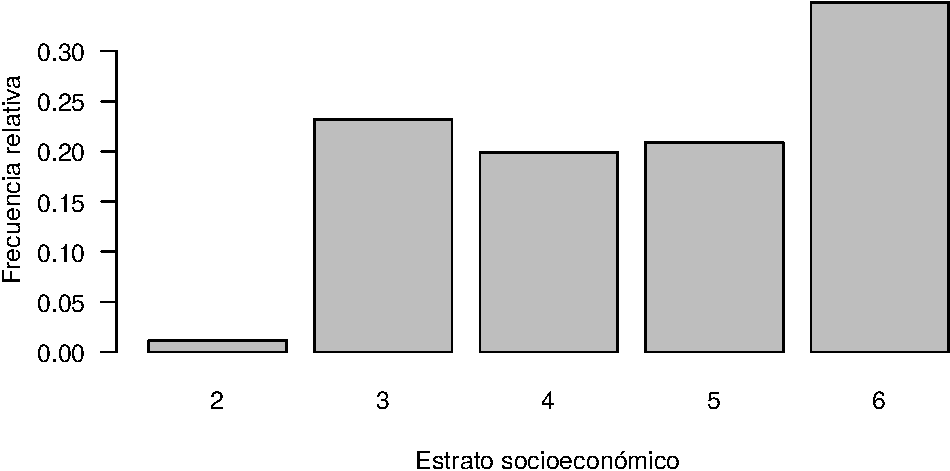
\includegraphics{Graficos_con_R_files/figure-latex/barra1-1.pdf}
\caption{\label{fig:barra1}Diagrama de barras para el estrato socioeconómico
de los apartamentos usados.}
\end{figure}

En la Figura \ref{fig:barra1} se presenta el diagrama de barras
solicitado. Se observa que hay pocos apartamentos (1.15\%)
pertenecientes al estrato dos, los estratos tres, cuatro y cinco aportan
porcentajes similares a la base de datos y que el estrato 6 es el que
más apartamentos aporta a la base de datos, 34.87\%.

Algunas veces se acostumbra a colocar las frecuencias relativas sobre la
parte superior de las barras para facilitar la lectura. A continuación
se presenta el código para replicar la Figura \ref{fig:barra1} con las
frecuencias relativas. Lo primero que se hace es dibujar el diagrama de
barras y almacenar la información de él en el objeto \texttt{xx} para
luego poder usar la ubicación de cada una de las barras. Note que se
agregó también \texttt{ylim=c(0,\ 0.45)} para conseguir una ampliación
del eje vertical, esto para lograr que se vea el número sobre la barra
del estrato 6. Luego se usa la función \texttt{text} para incluir un
texto en las coordenadas \texttt{x=xx} y \texttt{y=tabla1}, el parámetro
\texttt{pos=3} coloca el texto en la parte superior de las coordenadas y
el parámetro \texttt{label} sirve para indicar lo que se desea escribir
en las coordenadas indicadas, en este caso son las frecuencias relativas
almacenadas en \texttt{tabla1}.

\begin{Shaded}
\begin{Highlighting}[]
\NormalTok{xx <-}\StringTok{ }\KeywordTok{barplot}\NormalTok{(tabla1, }\DataTypeTok{ylim=}\KeywordTok{c}\NormalTok{(}\DecValTok{0}\NormalTok{, }\FloatTok{0.45}\NormalTok{), }\DataTypeTok{col=}\KeywordTok{gray}\NormalTok{(}\FloatTok{0.9}\NormalTok{),}
              \DataTypeTok{xlab=}\StringTok{'Estrato socioeconómico'}\NormalTok{,}
              \DataTypeTok{ylab=}\StringTok{'Frecuencia relativa'}\NormalTok{, }\DataTypeTok{las=}\DecValTok{1}\NormalTok{)}

\KeywordTok{text}\NormalTok{(}\DataTypeTok{x=}\NormalTok{xx, }\DataTypeTok{y=}\NormalTok{tabla1, }\DataTypeTok{pos=}\DecValTok{3}\NormalTok{, }\DataTypeTok{cex=}\FloatTok{0.8}\NormalTok{, }\DataTypeTok{col=}\StringTok{"red"}\NormalTok{,}
     \DataTypeTok{label=}\KeywordTok{round}\NormalTok{(tabla1, }\DecValTok{4}\NormalTok{))}
\end{Highlighting}
\end{Shaded}

\begin{figure}[htbp]
\centering
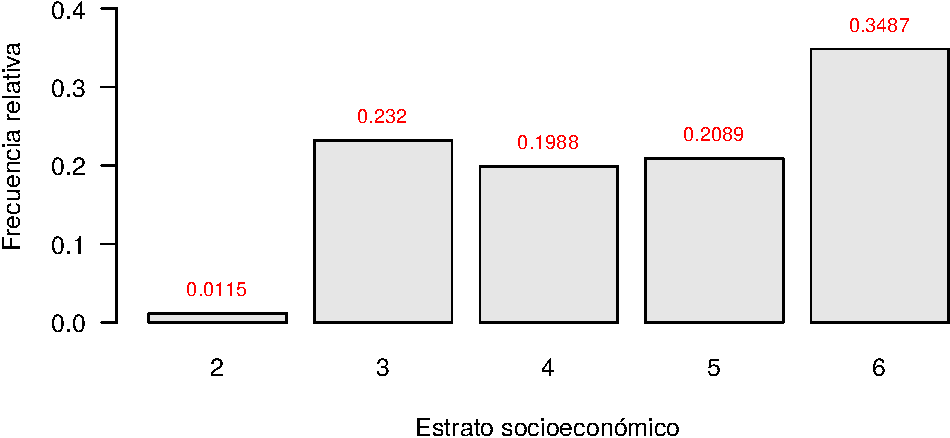
\includegraphics{Graficos_con_R_files/figure-latex/barra2-1.pdf}
\caption{\label{fig:barra2}Diagrama de barras para el estrato socioeconómico
de los apartamentos usados con las frecuencias relativas sobre las
barras.}
\end{figure}

En la Figura \ref{fig:barra2} se muestra el diagrama de barras
modificado. Note que si no se hubiese usado \texttt{ylim=c(0,\ 0.45)} al
dibujar el diagrama, la marca sobre la última barra no se podría ver.

\chapter{Gráficos para varias
variables}\label{graficos-para-varias-variables}

En este capítulo se presentan funciones para la creación de gráficos que
involucran varias variables.

\section{\texorpdfstring{Función \texttt{plot} \index{plot}
\index{diagrama de dispersión}}{Función plot  }}\label{funcion-plot}

Los gráficos de dispersión son muy útiles porque permiten ver la
relación que existe entre dos variables cuantitativas, la función
\texttt{plot} permite crear este tipo de gráficos. La estructura de la
función \texttt{plot} con los argumentos más usuales se muestran a
continuación

\begin{Shaded}
\begin{Highlighting}[]
\KeywordTok{plot}\NormalTok{(x, y, type, main, sub, xlab, ylab)}
\end{Highlighting}
\end{Shaded}

Los argumentos de la función \texttt{plot} son:

\begin{itemize}
\tightlist
\item
  \texttt{x}: vector numérico con las coordenadas del eje horizontal.
\item
  \texttt{y}: vector numérico con las coordenadas del eje vertical
\item
  \texttt{type}: tipo de gráfico a dibujar. Las opciones son:

  \begin{itemize}
  \tightlist
  \item
    \texttt{\textquotesingle{}p\textquotesingle{}} para obtener puntos,
    esta es la opción por defecto.
  \item
    \texttt{\textquotesingle{}l\textquotesingle{}} para obtener líneas.
  \item
    \texttt{\textquotesingle{}b\textquotesingle{}} para obtener los
    puntos y líneas que unen los puntos.
  \item
    \texttt{\textquotesingle{}c\textquotesingle{}} para obtener sólo las
    líneas y dejando los espacios donde estaban los puntos obtenidos con
    la opción \texttt{\textquotesingle{}b\textquotesingle{}}.
  \item
    \texttt{\textquotesingle{}o\textquotesingle{}} para obtener los
    puntos y lineas superpuestas.
  \item
    \texttt{\textquotesingle{}h\textquotesingle{}} para obtener líneas
    verticales desde el origen hasta el valor \(y_i\) de cada punto,
    similar a un histograma.
  \item
    \texttt{\textquotesingle{}s\textquotesingle{}} para obtener
    escalones.
  \item
    \texttt{\textquotesingle{}S\textquotesingle{}} similar al anterior.
  \item
    \texttt{\textquotesingle{}n\textquotesingle{}} para que no dibuje.
  \end{itemize}
\item
  \texttt{...}: otros parámetros gráficos que pueden ser pasados como
  argumentos para \texttt{plot}.
\end{itemize}

\subsection*{Ejemplo}\label{ejemplo-9}


Crear 16 parejas de puntos tales que \(x=-5, -4, \ldots, 9, 10\) con
\(y=-10+(x-3)^2\), dibujar los nueve diagramas de dispersión de \(y\)
contra \(x\) usando todos los valores posibles para el parámetro
\texttt{type}.

A continuación se muestra el código para crear las 16 parejas de \(x\) e
\(y\). Los nueve diagramas de dispersión se observan en la Figura
\ref{fig:ex1plot}, de esta figura se observa claramente el efecto que
tiene el parámetro \texttt{type} en la construcción del diagrama de
dispersión.

\begin{Shaded}
\begin{Highlighting}[]
\NormalTok{x <-}\StringTok{ }\NormalTok{-}\DecValTok{5}\NormalTok{:}\DecValTok{10}
\NormalTok{y <-}\StringTok{ }\NormalTok{-}\DecValTok{10} \NormalTok{+}\StringTok{ }\NormalTok{(x}\DecValTok{-3}\NormalTok{)^}\DecValTok{2}
\KeywordTok{par}\NormalTok{(}\DataTypeTok{mfrow=}\KeywordTok{c}\NormalTok{(}\DecValTok{3}\NormalTok{, }\DecValTok{3}\NormalTok{))}
\KeywordTok{plot}\NormalTok{(}\DataTypeTok{x=}\NormalTok{x, }\DataTypeTok{y=}\NormalTok{y, }\DataTypeTok{type=}\StringTok{'p'}\NormalTok{, }\DataTypeTok{main=}\StringTok{"con type='p'"}\NormalTok{)}
\KeywordTok{plot}\NormalTok{(}\DataTypeTok{x=}\NormalTok{x, }\DataTypeTok{y=}\NormalTok{y, }\DataTypeTok{type=}\StringTok{'l'}\NormalTok{, }\DataTypeTok{main=}\StringTok{"con type='l'"}\NormalTok{)}
\KeywordTok{plot}\NormalTok{(}\DataTypeTok{x=}\NormalTok{x, }\DataTypeTok{y=}\NormalTok{y, }\DataTypeTok{type=}\StringTok{'b'}\NormalTok{, }\DataTypeTok{main=}\StringTok{"con type='b'"}\NormalTok{)}
\KeywordTok{plot}\NormalTok{(}\DataTypeTok{x=}\NormalTok{x, }\DataTypeTok{y=}\NormalTok{y, }\DataTypeTok{type=}\StringTok{'c'}\NormalTok{, }\DataTypeTok{main=}\StringTok{"con type='c'"}\NormalTok{)}
\KeywordTok{plot}\NormalTok{(}\DataTypeTok{x=}\NormalTok{x, }\DataTypeTok{y=}\NormalTok{y, }\DataTypeTok{type=}\StringTok{'o'}\NormalTok{, }\DataTypeTok{main=}\StringTok{"con type='o'"}\NormalTok{)}
\KeywordTok{plot}\NormalTok{(}\DataTypeTok{x=}\NormalTok{x, }\DataTypeTok{y=}\NormalTok{y, }\DataTypeTok{type=}\StringTok{'h'}\NormalTok{, }\DataTypeTok{main=}\StringTok{"con type='h'"}\NormalTok{)}
\KeywordTok{plot}\NormalTok{(}\DataTypeTok{x=}\NormalTok{x, }\DataTypeTok{y=}\NormalTok{y, }\DataTypeTok{type=}\StringTok{'s'}\NormalTok{, }\DataTypeTok{main=}\StringTok{"con type='s'"}\NormalTok{)}
\KeywordTok{plot}\NormalTok{(}\DataTypeTok{x=}\NormalTok{x, }\DataTypeTok{y=}\NormalTok{y, }\DataTypeTok{type=}\StringTok{'S'}\NormalTok{, }\DataTypeTok{main=}\StringTok{"con type='S'"}\NormalTok{)}
\KeywordTok{plot}\NormalTok{(}\DataTypeTok{x=}\NormalTok{x, }\DataTypeTok{y=}\NormalTok{y, }\DataTypeTok{type=}\StringTok{'n'}\NormalTok{, }\DataTypeTok{main=}\StringTok{"con type='n'"}\NormalTok{)}
\end{Highlighting}
\end{Shaded}

\begin{figure}[htbp]
\centering
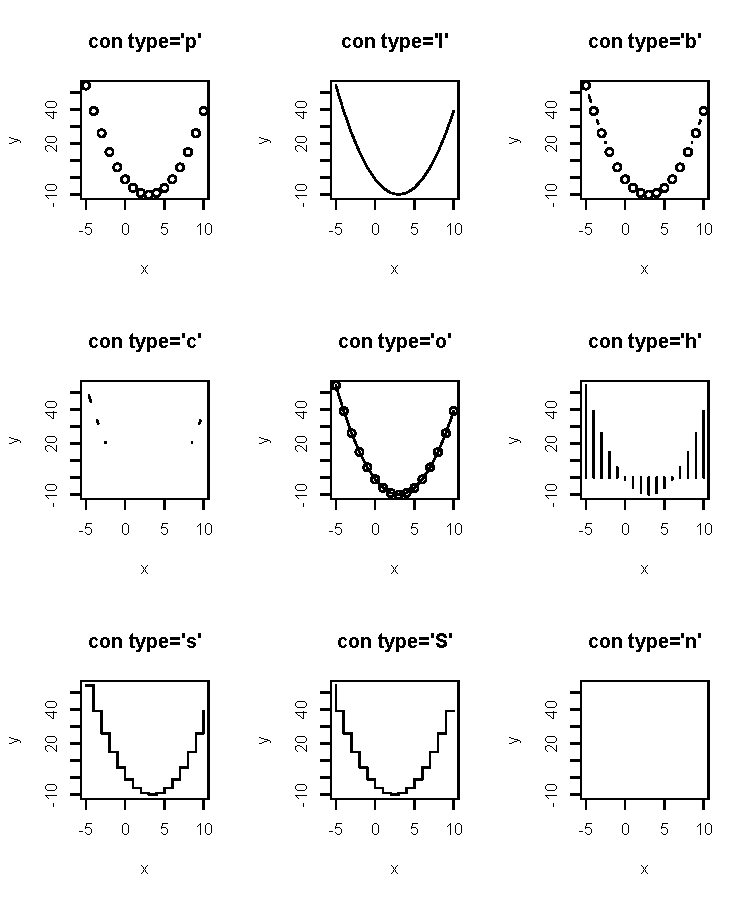
\includegraphics{Graficos_con_R_files/figure-latex/ex1plot-1.pdf}
\caption{\label{fig:ex1plot}Efecto del parámetro \texttt{type} en la función
\texttt{plot}.}
\end{figure}

\subsection*{Ejemplo}\label{ejemplo-10}


Como ilustración vamos a crear un diagrama de dispersión entre el precio
de apartamentos usados en la ciudad de Medellín y el área de los
apartamentos. El código necesario para cargar la base de datos y
construir el diagrama de dispersión se muestra a continuación.

\begin{Shaded}
\begin{Highlighting}[]
\NormalTok{url <-}\StringTok{ 'https://raw.githubusercontent.com/fhernanb/datos/master/aptos2015'}
\NormalTok{datos <-}\StringTok{ }\KeywordTok{read.table}\NormalTok{(}\DataTypeTok{file=}\NormalTok{url, }\DataTypeTok{header=}\NormalTok{T)}

\KeywordTok{par}\NormalTok{(}\DataTypeTok{mfrow=}\KeywordTok{c}\NormalTok{(}\DecValTok{1}\NormalTok{, }\DecValTok{2}\NormalTok{))}
\KeywordTok{plot}\NormalTok{(}\DataTypeTok{x=}\NormalTok{datos$mt2, }\DataTypeTok{y=}\NormalTok{datos$precio)}
\KeywordTok{plot}\NormalTok{(}\DataTypeTok{x=}\NormalTok{datos$mt2, }\DataTypeTok{y=}\NormalTok{datos$precio, }\DataTypeTok{pch=}\StringTok{'.'}\NormalTok{,}
     \DataTypeTok{xlab=}\StringTok{'Área del apartamento (m2)'}\NormalTok{, }\DataTypeTok{ylab=}\StringTok{'Precio (millones de pesos)'}\NormalTok{)}
\end{Highlighting}
\end{Shaded}

\begin{figure}[htbp]
\centering
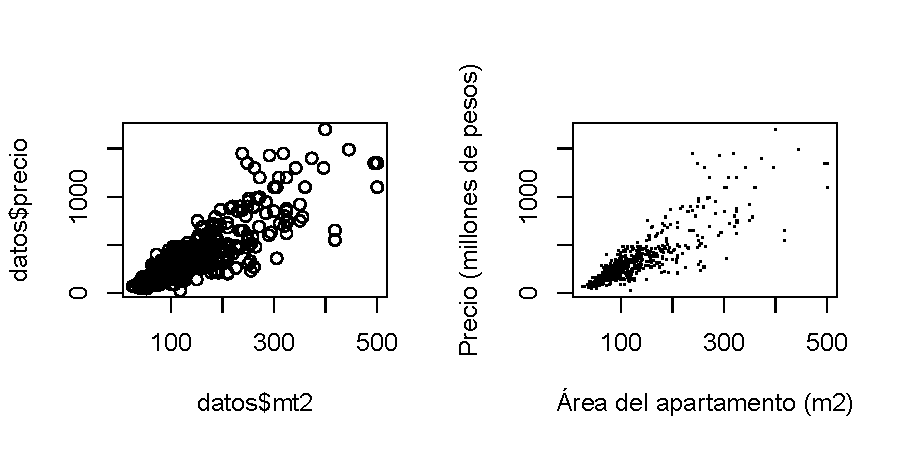
\includegraphics{Graficos_con_R_files/figure-latex/ex2plot-1.pdf}
\caption{\label{fig:ex2plot}Diagrama de dispersión del precio del
apartamento versus área del apartamento. A la izquierda el diagrama de
dispersión sin editar y a la derecha el diagrama de dispersión mejorado}
\end{figure}

En la Figura \ref{fig:ex2plot} se presenta el diagrama de dispersión
entre precio y área de los apartamentos, de este diagrama se observa
claramente que a medida que los apartamentos tienen mayor área el precio
promedio y la variabilidad del precio aumentan. Para el diagrama de
dispersión de la derecha se usó el parámetro
\texttt{pch=\textquotesingle{}.\textquotesingle{}} con el objetivo de
obtener pequeños puntos que representen cada apartamento y que no se
traslapen debido a que se tienen 694 observaciones en la base de datos.

\section{\texorpdfstring{Función \texttt{persp}
\index{persp}}{Función persp }}\label{funcion-persp}

La función \texttt{persp} dibuja superfices en tres dimensiones y es
posible rotar la superficie para obtener una perpectiva apropiada. La
estructura de la función \texttt{persp} con los argumentos más usuales
se muestran a continuación.

\begin{Shaded}
\begin{Highlighting}[]
\KeywordTok{persp}\NormalTok{(x, y, z, main, sub, theta, phi, r, col, border, box, axes, nticks)}
\end{Highlighting}
\end{Shaded}

Los argumentos de la función \texttt{plot} son:

\begin{itemize}
\tightlist
\item
  \texttt{x}: vector numérico con los valores de \(x\) donde fue
  evaluada la función o superficie.
\item
  \texttt{y}: vector numérico con los valores de \(y\) donde fue
  evaluada la función o superficie.
\item
  \texttt{z}: matriz que contiene las alturas \(z\) de la supercifie
  para cada combinación de \(x\) e \(y\).
\item
  \texttt{main}: vector numérico con las coordenadas del eje vertical.
\item
  \texttt{sub}: vector numérico con las coordenadas del eje vertical.
\item
  \texttt{theta,\ phi}: ángulo para la visión de la superficie,
  \texttt{theta} para la dirección azimutal y \texttt{phi} para latitud.
  Ver Figura \ref{fig:globo} para una ilustración de los ángulos.
\item
  \texttt{r}: distancia entre el centro de la caja de dibujo al punto de
  vista.
\item
  \texttt{col}: color de la superficie.
\item
  \texttt{border}: color para el borde de la superficie.
\item
  \texttt{box}: valor lógico para indicar si se quiere dibujar la caja
  que contiene la superficie, por defecto es \texttt{TRUE}.
\item
  \texttt{axes}: valor lógico para indicar si se desean marcas en los
  ejes y nombres de los ejes, por defecto es \texttt{TRUE}. Si
  \texttt{box=\textquotesingle{}FALSE\textquotesingle{}} no aparecen
  marcas ni nombres de los ejes.
\item
  \texttt{expand}: factor de expansión aplicado a los valores en el eje
  \texttt{z}.
\item
  \texttt{ticktype}: tipo de marcas a colocar en los ejes,
  \texttt{simple} no dibuja nada y \texttt{detailed} coloca números a
  los ejes.
\item
  \texttt{nticks}: número aproximado de marcas en los ejes.
\end{itemize}

\begin{figure}

{\centering 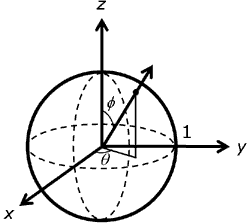
\includegraphics[width=0.25\linewidth]{images/IC412528} 

}

\caption{Ilustración de los angulos theta y phi para la función persp. Figura tomada de https://i-msdn.sec.s-msft.com/dynimg/IC412528.png}\label{fig:globo}
\end{figure}

\subsection*{Ejemplo}\label{ejemplo-11}


Dibujar la superficie asociada a la función \(f(x, y)=sen(x^2+y^2)\)
para \(-2 \leq x \leq2\) y \(-2 \leq y \leq2\). Usar 4 combinaciones de
los parámetros \texttt{theta} y \texttt{phi} para obtener un buen punto
de vista de la superficie.

Lo primero que se debe hacer es crear la función \(f(x, y)\) la cual se
va a llamar \texttt{fun}. Luego se definen los vectores \texttt{x} e
\texttt{y} tomando por ejemplo 25 puntos equiespaciados en el intervalo
\([-2, 2]\). Luego se usa la función \texttt{outer} para crear la
rejilla o matriz que contiene los valores de \(f(x, y)\) para cada
combinación de \texttt{x} e \texttt{y}, los resultados se almacenan en
el objeto \texttt{z}. Por último se dibujan 4 perspectivas de la función
variando los parámetros \texttt{theta} y \texttt{phi} de la función
\texttt{persp}. A continuación el código utilizado.

\begin{Shaded}
\begin{Highlighting}[]
\NormalTok{fun <-}\StringTok{ }\NormalTok{function(x, y)   }\KeywordTok{sin}\NormalTok{(x^}\DecValTok{2} \NormalTok{+}\StringTok{ }\NormalTok{y^}\DecValTok{2}\NormalTok{)}
\NormalTok{x <-}\StringTok{ }\KeywordTok{seq}\NormalTok{(}\DataTypeTok{from=}\NormalTok{-}\DecValTok{2}\NormalTok{, }\DataTypeTok{to=}\DecValTok{2}\NormalTok{, }\DataTypeTok{length.out=}\DecValTok{25}\NormalTok{)}
\NormalTok{y <-}\StringTok{ }\KeywordTok{seq}\NormalTok{(}\DataTypeTok{from=}\NormalTok{-}\DecValTok{2}\NormalTok{, }\DataTypeTok{to=}\DecValTok{2}\NormalTok{, }\DataTypeTok{length.out=}\DecValTok{25}\NormalTok{)}
\NormalTok{z <-}\StringTok{ }\KeywordTok{outer}\NormalTok{(x, y, fun)}

\KeywordTok{par}\NormalTok{(}\DataTypeTok{mfrow=}\KeywordTok{c}\NormalTok{(}\DecValTok{2}\NormalTok{, }\DecValTok{2}\NormalTok{), }\DataTypeTok{mar=}\KeywordTok{c}\NormalTok{(}\DecValTok{1}\NormalTok{, }\DecValTok{1}\NormalTok{, }\DecValTok{2}\NormalTok{, }\DecValTok{1}\NormalTok{))}
\KeywordTok{persp}\NormalTok{(x, y, z, }\DataTypeTok{zlim=}\KeywordTok{c}\NormalTok{(-}\DecValTok{1}\NormalTok{, }\FloatTok{1.5}\NormalTok{), }\DataTypeTok{theta=}\DecValTok{0}\NormalTok{, }\DataTypeTok{phi=}\DecValTok{0}\NormalTok{, }\DataTypeTok{col=}\StringTok{'aquamarine'}\NormalTok{,}
      \DataTypeTok{main=}\StringTok{'(A) theta=0, phi=0'}\NormalTok{)}
\KeywordTok{persp}\NormalTok{(x, y, z, }\DataTypeTok{zlim=}\KeywordTok{c}\NormalTok{(-}\DecValTok{1}\NormalTok{, }\FloatTok{1.5}\NormalTok{), }\DataTypeTok{theta=}\DecValTok{15}\NormalTok{, }\DataTypeTok{phi=}\DecValTok{15}\NormalTok{, }\DataTypeTok{col=}\StringTok{'lightpink'}\NormalTok{,}
      \DataTypeTok{main=}\StringTok{'(B) theta=15, phi=15'}\NormalTok{)}
\KeywordTok{persp}\NormalTok{(x, y, z, }\DataTypeTok{zlim=}\KeywordTok{c}\NormalTok{(-}\DecValTok{1}\NormalTok{, }\FloatTok{1.5}\NormalTok{), }\DataTypeTok{theta=}\DecValTok{45}\NormalTok{, }\DataTypeTok{phi=}\DecValTok{30}\NormalTok{, }\DataTypeTok{col=}\StringTok{'yellow1'}\NormalTok{,}
      \DataTypeTok{main=}\StringTok{'(c) theta=45, phi=30'}\NormalTok{)}
\KeywordTok{persp}\NormalTok{(x, y, z, }\DataTypeTok{zlim=}\KeywordTok{c}\NormalTok{(-}\DecValTok{1}\NormalTok{, }\FloatTok{1.5}\NormalTok{), }\DataTypeTok{theta=}\DecValTok{60}\NormalTok{, }\DataTypeTok{phi=}\DecValTok{50}\NormalTok{, }\DataTypeTok{col=}\StringTok{'lightblue'}\NormalTok{,}
      \DataTypeTok{main=}\StringTok{'(D) theta=60, phi=50'}\NormalTok{)}
\end{Highlighting}
\end{Shaded}

\begin{figure}[htbp]
\centering
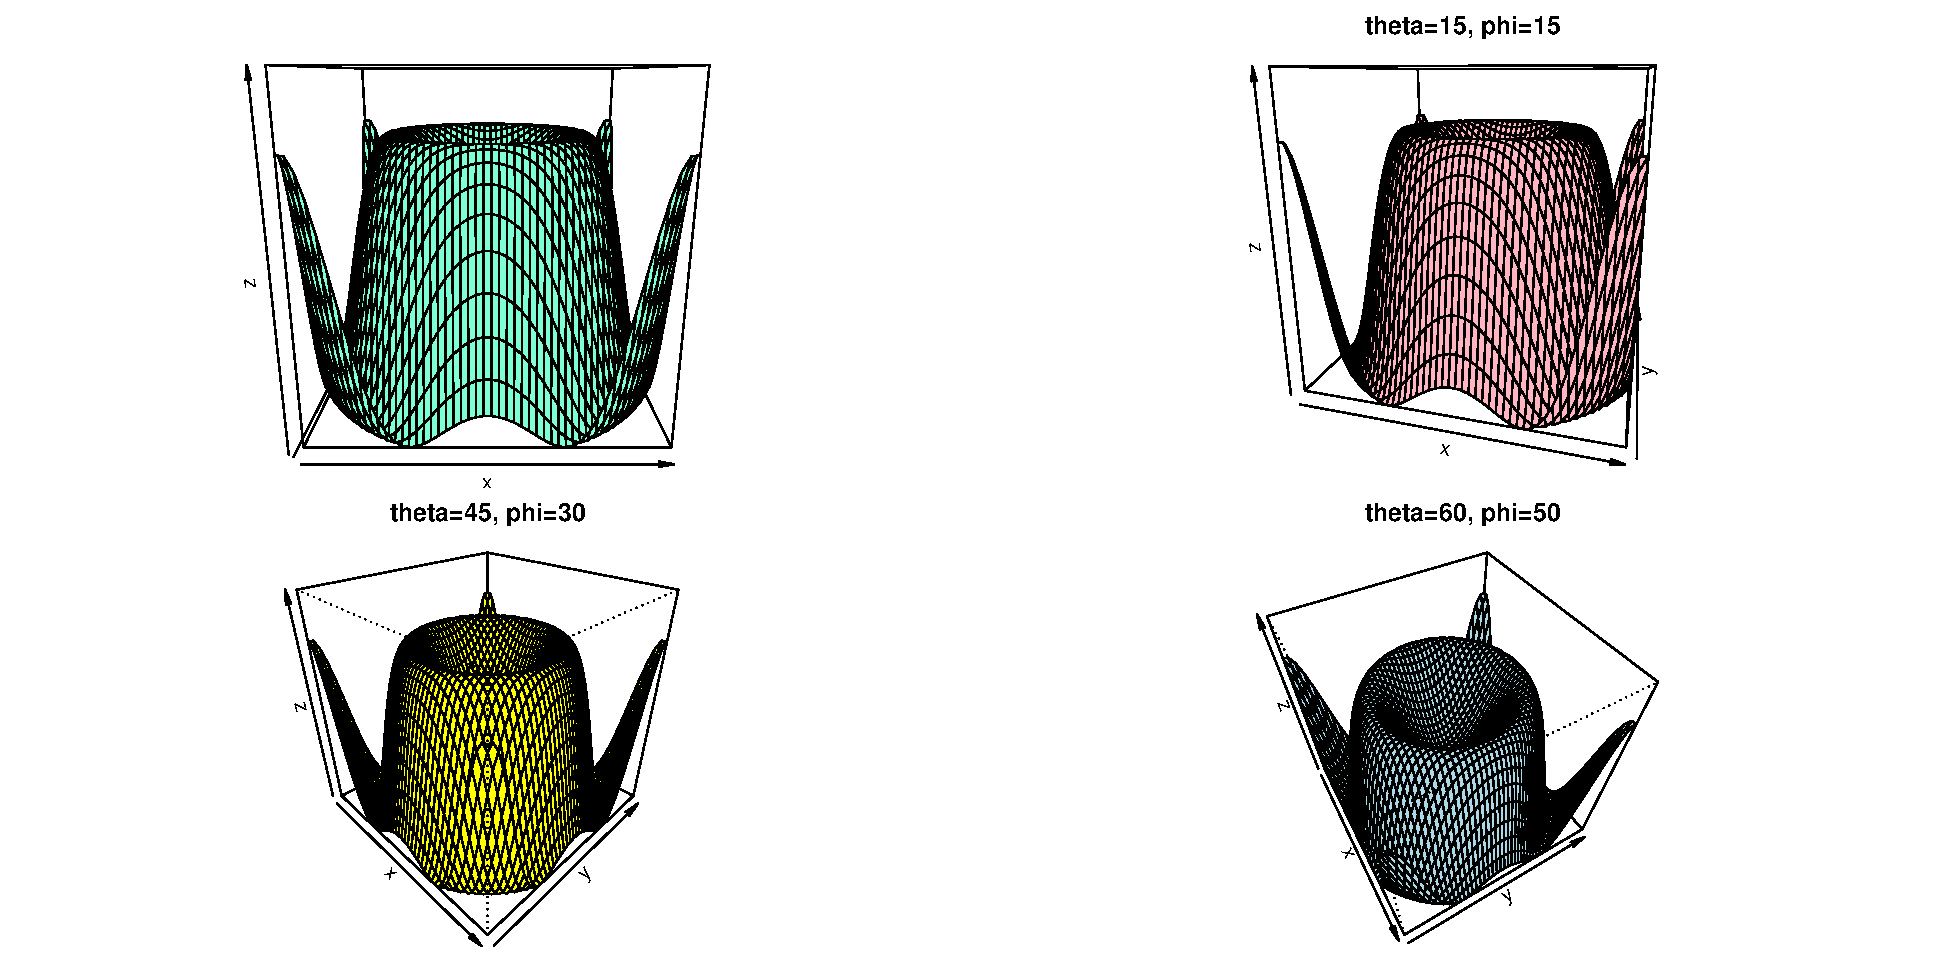
\includegraphics{Graficos_con_R_files/figure-latex/ex1persp-1.pdf}
\caption{\label{fig:ex1persp}Superficie generada con \texttt{persp} y
diferentes valores de theta y phi.}
\end{figure}

En la Figura \ref{fig:ex1persp} se presentan las 4 perspectivas de la
función \(f(x, y)=sen(x^2+y^2)\). De los 4 páneles se nota que (C) y (D)
muestran mejor la superficie de interés.

Al aumentar el valor del parámetro \texttt{length.out} en la creación de
los vectores \texttt{x} e \texttt{y} se obtendrá una rejilla más tupida,
se recomienda modificar este valor para obtener una superficie
apropiada.

\subsection*{Ejemplo}\label{ejemplo-12}


Dibujar la superficie de una distribución normal bivariada con vector de
medias \(\boldsymbol{\mu}=(5, 12)^\top\), varianzas unitarias y
covarianza con valor de -0.8. Explorar el efecto de los parámetros
\texttt{ticktype}, \texttt{nticks}, \texttt{expand}, \texttt{axes} y
\texttt{box}.

Primero se define el vector de medias y la matriz de varianzas y
covarianzas, luego se carga el paquete \texttt{mvtnorm} que contiene la
función \texttt{dmvnorm} que calcula la densidad dado el vector de
medias y la matriz de varianzas y covarianzas. Se construye la función
\texttt{fun} y se vectoriza para luego obtener las alturas de la
superficie con la ayuda de \texttt{outer}. Por último se dibujan tres
perspectivas diferentes para la densidad modificando los parámetros
\texttt{ticktype}, \texttt{nticks}, \texttt{expand}, \texttt{axes} y
\texttt{box}, a continuación el código usado.

\begin{Shaded}
\begin{Highlighting}[]
\NormalTok{media <-}\StringTok{ }\KeywordTok{c}\NormalTok{(}\DecValTok{5}\NormalTok{, }\DecValTok{12}\NormalTok{)}
\NormalTok{varianza <-}\StringTok{ }\KeywordTok{matrix}\NormalTok{(}\KeywordTok{c}\NormalTok{(}\DecValTok{1}\NormalTok{, -}\FloatTok{0.8}\NormalTok{, -}\FloatTok{0.8}\NormalTok{, }\DecValTok{1}\NormalTok{), }\DataTypeTok{ncol=}\DecValTok{2}\NormalTok{)}

\KeywordTok{require}\NormalTok{(mvtnorm)}
\NormalTok{fun <-}\StringTok{ }\NormalTok{function(x, y) }\KeywordTok{dmvnorm}\NormalTok{(}\KeywordTok{c}\NormalTok{(x, y), }\DataTypeTok{mean=}\NormalTok{media, }\DataTypeTok{sigma=}\NormalTok{varianza)}
\NormalTok{fun <-}\StringTok{ }\KeywordTok{Vectorize}\NormalTok{(fun)}

\NormalTok{x <-}\StringTok{ }\KeywordTok{seq}\NormalTok{(}\DataTypeTok{from=}\DecValTok{2}\NormalTok{, }\DataTypeTok{to=}\DecValTok{8}\NormalTok{, }\DataTypeTok{length.out=}\DecValTok{30}\NormalTok{)}
\NormalTok{y <-}\StringTok{ }\KeywordTok{seq}\NormalTok{(}\DataTypeTok{from=}\DecValTok{9}\NormalTok{, }\DataTypeTok{to=}\DecValTok{15}\NormalTok{, }\DataTypeTok{length.out=}\DecValTok{30}\NormalTok{)}
\NormalTok{z <-}\StringTok{ }\KeywordTok{outer}\NormalTok{(x, y, fun)}

\KeywordTok{par}\NormalTok{(}\DataTypeTok{mfrow=}\KeywordTok{c}\NormalTok{(}\DecValTok{1}\NormalTok{, }\DecValTok{3}\NormalTok{), }\DataTypeTok{mar=}\KeywordTok{c}\NormalTok{(}\DecValTok{1}\NormalTok{, }\DecValTok{1}\NormalTok{, }\DecValTok{2}\NormalTok{, }\DecValTok{1}\NormalTok{))}
\KeywordTok{persp}\NormalTok{(x, y, z, }\DataTypeTok{theta=}\DecValTok{30}\NormalTok{, }\DataTypeTok{phi=}\DecValTok{30}\NormalTok{, }\DataTypeTok{ticktype =} \StringTok{"detailed"}\NormalTok{, }\DataTypeTok{nticks=}\DecValTok{4}\NormalTok{)}
\KeywordTok{persp}\NormalTok{(x, y, z, }\DataTypeTok{theta=}\DecValTok{30}\NormalTok{, }\DataTypeTok{phi=}\DecValTok{30}\NormalTok{, }\DataTypeTok{col=}\StringTok{'salmon1'}\NormalTok{, }\DataTypeTok{expand=}\FloatTok{0.5}\NormalTok{, }\DataTypeTok{axes=}\OtherTok{FALSE}\NormalTok{)}
\KeywordTok{persp}\NormalTok{(x, y, z, }\DataTypeTok{theta=}\DecValTok{30}\NormalTok{, }\DataTypeTok{phi=}\DecValTok{30}\NormalTok{, }\DataTypeTok{col=}\StringTok{'springgreen1'}\NormalTok{, }\DataTypeTok{expand=}\FloatTok{0.2}\NormalTok{, }\DataTypeTok{box=}\OtherTok{FALSE}\NormalTok{)}
\end{Highlighting}
\end{Shaded}

\begin{figure}[htbp]
\centering
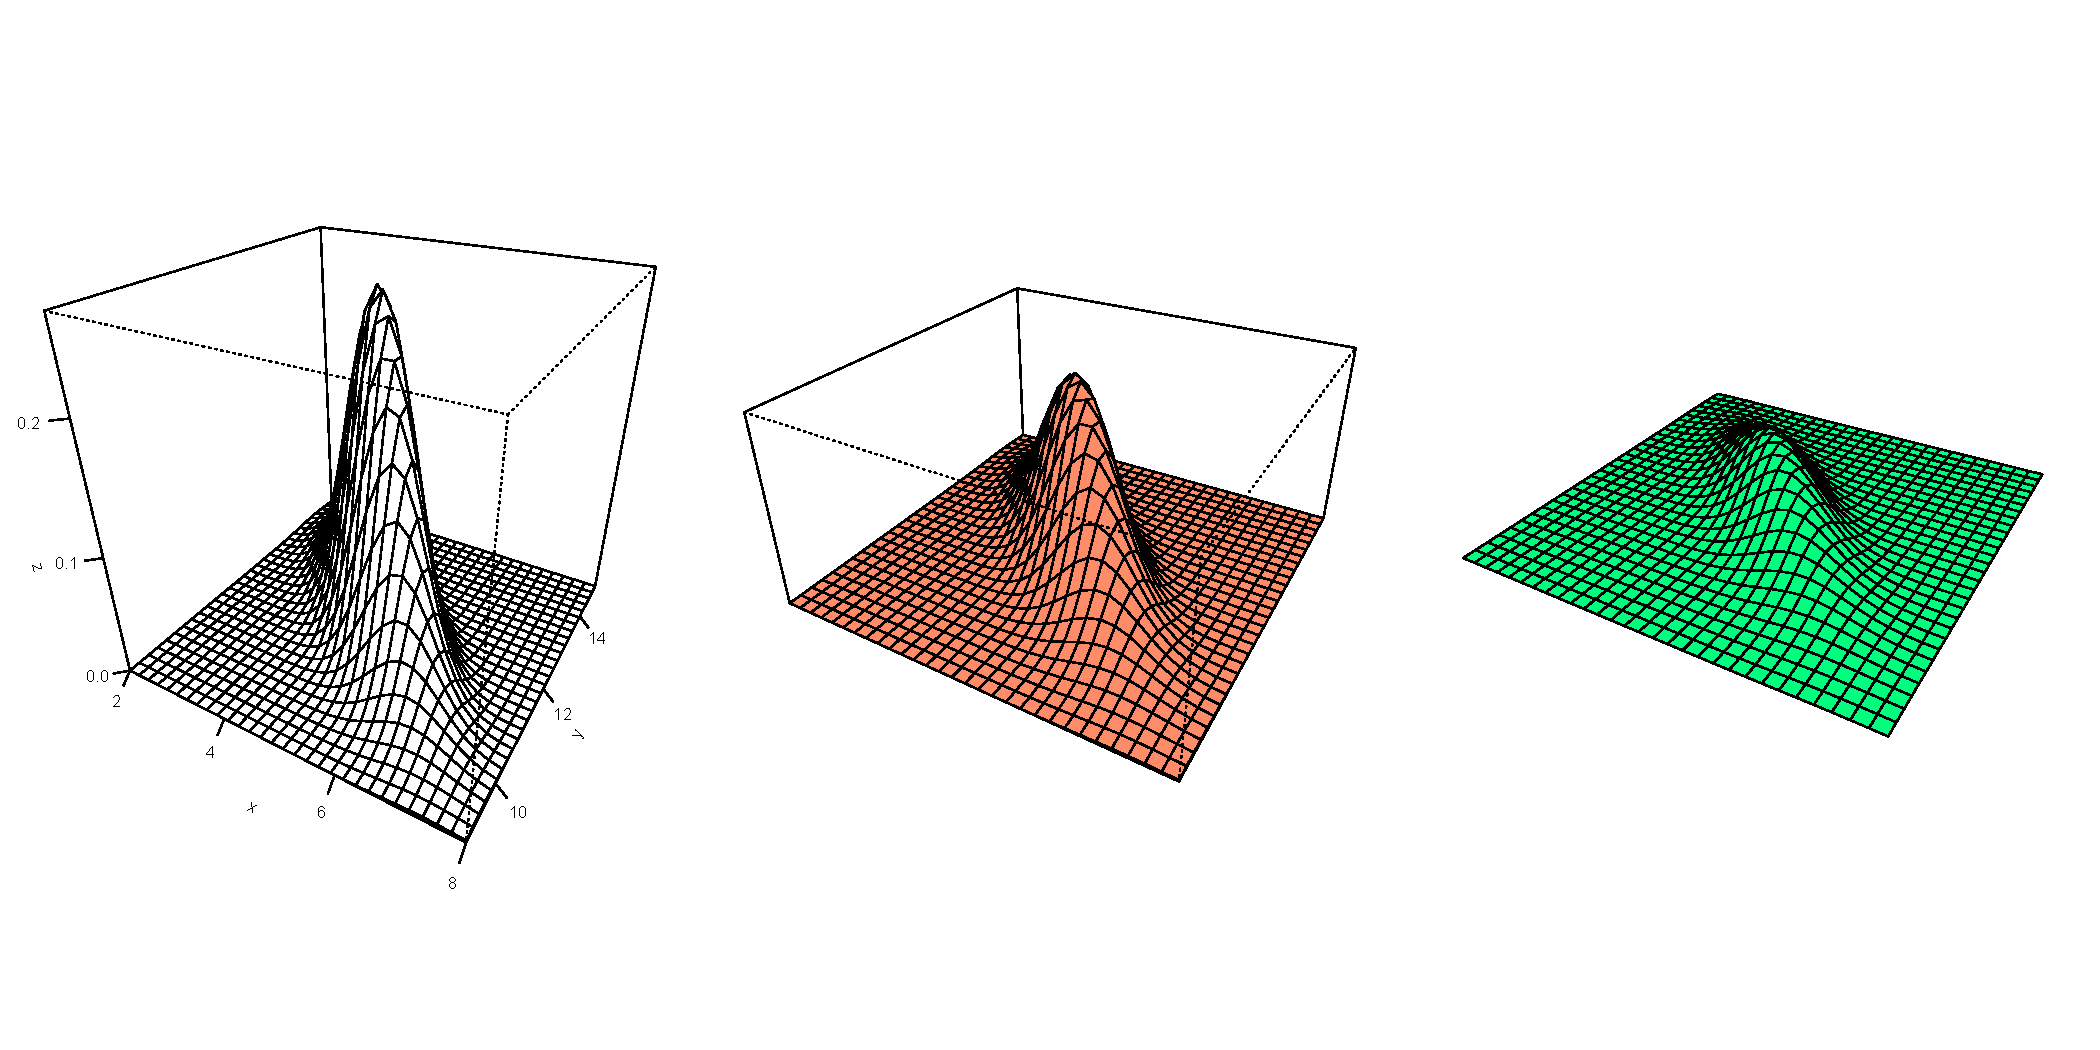
\includegraphics{Graficos_con_R_files/figure-latex/ex2persp-1.pdf}
\caption{\label{fig:ex2persp}Distribución normal bivariada.}
\end{figure}

En la Figura \ref{fig:ex2persp} se presentan las 3 perspectivas para la
densidad. Note los efectos que \texttt{ticktype}, \texttt{nticks},
\texttt{expand}, \texttt{axes} y \texttt{box} tienen sobre los dibujos
de las perspectivas.

\section{\texorpdfstring{Función \texttt{pairs}
\index{pairs}}{Función pairs }}\label{funcion-pairs}

Las matrices de dispersión obtenidas con la función \texttt{pairs}
proporcionan un método simple de presentar las relaciones entre pares de
variables cuantitativas y son la versión múltiple de la función
\texttt{plot}. Este gráfico consiste en una matriz donde cada entrada
presenta un gráfico de dispersión sencillo. Un inconveniente es que si
tenemos muchas variables el tamaño de cada entrada se reduce demasiado
impidiendo ver con claridad las relaciones entre los pares de variables.
La celda \((i,j)\) de una matriz de dispersión contiene el gráfico de
dispersión de la columna \(i\) versus la columna \(j\) de la matriz de
datos.

En la Figura \ref{fig:ex0pairs} se muestra un ejemplo de una matriz de
dispersión para un conjunto de datos, en la diagonal están los nombres
de las variables y por fuera de la diagonal están los diagramas de
dispersión para cada combinación de variables.

\begin{figure}[htbp]
\centering
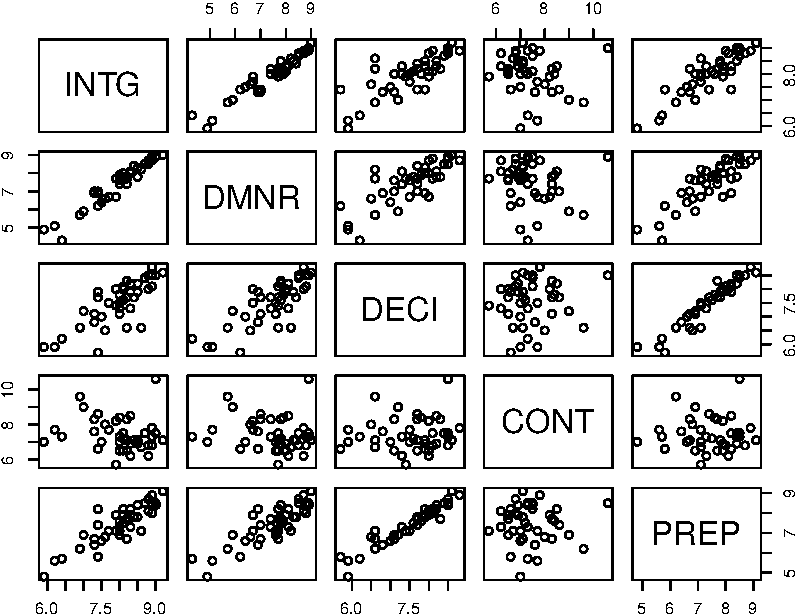
\includegraphics{Graficos_con_R_files/figure-latex/ex0pairs-1.pdf}
\caption{\label{fig:ex0pairs}Ilustración de una matriz de dispersión.}
\end{figure}

La estructura de la función \texttt{pairs} con los argumentos más
usuales se muestran a continuación.

\begin{Shaded}
\begin{Highlighting}[]
\KeywordTok{pairs}\NormalTok{(x, labels, }\DataTypeTok{panel =} \NormalTok{points, ...,}
      \DataTypeTok{horInd =} \DecValTok{1}\NormalTok{:nc, }\DataTypeTok{verInd =} \DecValTok{1}\NormalTok{:nc,}
      \DataTypeTok{lower.panel =} \NormalTok{panel, }\DataTypeTok{upper.panel =} \NormalTok{panel,}
      \DataTypeTok{diag.panel =} \OtherTok{NULL}\NormalTok{, }\DataTypeTok{text.panel =} \NormalTok{textPanel,}
      \DataTypeTok{label.pos =} \FloatTok{0.5} \NormalTok{+}\StringTok{ }\NormalTok{has.diag/}\DecValTok{3}\NormalTok{, }\DataTypeTok{line.main =} \DecValTok{3}\NormalTok{,}
      \DataTypeTok{cex.labels =} \OtherTok{NULL}\NormalTok{, }\DataTypeTok{font.labels =} \DecValTok{1}\NormalTok{,}
      \DataTypeTok{row1attop =} \OtherTok{TRUE}\NormalTok{, }\DataTypeTok{gap =} \DecValTok{1}\NormalTok{, }\DataTypeTok{log =} \StringTok{""}\NormalTok{)}
\end{Highlighting}
\end{Shaded}

Los argumentos de la función \texttt{pairs} son:

\begin{itemize}
\tightlist
\item
  \texttt{x}: matriz o marco de datos con la información de las
  variables cuantitativas a incluir en la matriz de dispersión.
\item
  \texttt{labels}: vector opcional con los nombres a colocar en la
  diagonal, por defecto se usan los nombres de columnas del objeto
  \texttt{x}.
\item
  \texttt{panel}: función usual de la forma \texttt{function(x,y,...)} a
  ser usada para determinar el contenido de los páneles. Por defecto es
  \texttt{points}, indicando que se graficarán los puntos de los pares
  de variables. Es posible utilizar aquí otras funciones diseñadas por
  el usuario.
\item
  \texttt{...}: Indica que es posible agregar otros parámetros gráficos,
  tales como \texttt{pch} y \texttt{col}, con los cuales puede
  especificarse un vector de símbolos y colores a ser usados en los
  scatterplots.
\item
  \texttt{lower.panel,\ upper.panel}: función usual de la forma
  \texttt{function(x,y,...)} para definir lo que se desea dibujar en los
  paneles abajo y arriba de la diagonal.
\item
  \texttt{diag.panel}: función usual de la forma
  \texttt{function(x,y,...)} para definir lo que se desea dibujar en la
  diagonal.
\item
  \texttt{text.panel}: Es opcional. Permite que una función:
  \texttt{function(x,\ y,\ labels,\ cex,\ font,\ ...)} sea aplicada a
  los paneles de la diagonal.
\item
  \texttt{label.pos}: Para especificar la posición \(y\) de las
  etiquetas en el text panel.
\item
  \texttt{cex.labels,\ font.labels}: Parámetros para la expansión de
  caracteres y fuentes a usar en las etiquetas de las variables.
\item
  \texttt{row1attop}: Parámetro lógico con el cual se especifica si el
  gráfico para especificar si el diseño lucirá como una matriz con su
  primera fila en la parte superior o como un gráfico con fila uno en la
  base. Por defecto es lo primero.
\end{itemize}

\subsection*{Ejemplo}\label{ejemplo-13}


Dibujar una matriz de dispersión para las variables precio, área, número
de alcobas y número de baños de la base de datos sobre apartamentos en
Medellín.

A continuación se muestra el código usado para crear el gráfico
solicitado. El objeto \texttt{datos} corresponde a la base de datos
completa mientras que \texttt{datos.num} es el marco de datos sólo con
las variables de interés precio, área, número de alcobas y número de
baños.

\begin{Shaded}
\begin{Highlighting}[]
\NormalTok{url <-}\StringTok{ 'https://raw.githubusercontent.com/fhernanb/datos/master/aptos2015'}
\NormalTok{datos <-}\StringTok{ }\KeywordTok{read.table}\NormalTok{(}\DataTypeTok{file=}\NormalTok{url, }\DataTypeTok{header=}\NormalTok{T)}
\NormalTok{datos.num <-}\StringTok{ }\NormalTok{datos[, }\KeywordTok{c}\NormalTok{(}\StringTok{'precio'}\NormalTok{, }\StringTok{'mt2'}\NormalTok{, }\StringTok{'alcobas'}\NormalTok{, }\StringTok{'banos'}\NormalTok{)]}

\KeywordTok{pairs}\NormalTok{(datos.num)}
\end{Highlighting}
\end{Shaded}

\begin{figure}[htbp]
\centering
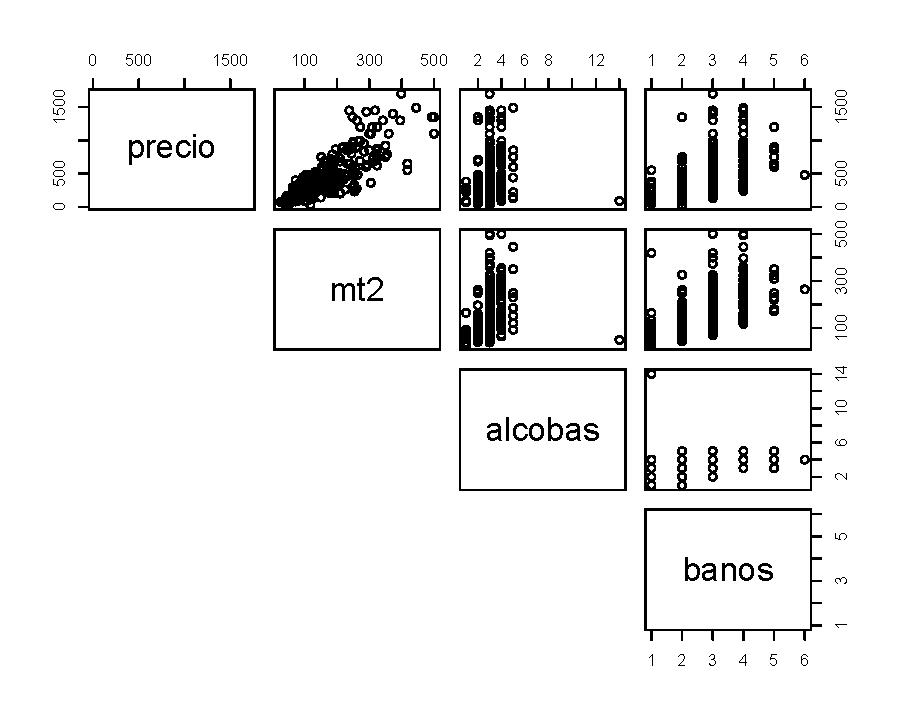
\includegraphics{Graficos_con_R_files/figure-latex/ex1pairs-1.pdf}
\caption{\label{fig:ex1pairs}Matriz de dispersión para las variables precio,
área, número de alcobas y número de baños de la base de datos sobre
apartamentos en Medellín.}
\end{figure}

En la Figura \ref{fig:ex1pairs} se muestra la matriz de dispersión para
las variables del marco de datos \texttt{datos.num}.

\subsection*{Ejemplo}\label{ejemplo-14}


Volver a construir la Figura \ref{fig:ex1pairs} editando los nombres de
las variables, usando cruces rojas en lugar de puntos, en escala
logaritmica, con marcas horizontales en el eje vertical y eliminando los
diagramas de dispersión abajo de la diagonal.

Para obtener la nueva matriz de dispersión con los cambios solicitados
se usa el siguiente código. En la Figura \ref{fig:ex2pairs} se presenta
la nueva matriz de dispersión.

\begin{Shaded}
\begin{Highlighting}[]
\KeywordTok{pairs}\NormalTok{(datos.num, }\DataTypeTok{lower.panel=}\OtherTok{NULL}\NormalTok{, }\DataTypeTok{cex.labels=}\FloatTok{1.5}\NormalTok{, }\DataTypeTok{log=}\StringTok{'xy'}\NormalTok{,}
      \DataTypeTok{main=}\StringTok{'Matriz de dispersión'}\NormalTok{, }\DataTypeTok{las=}\DecValTok{1}\NormalTok{,}
      \DataTypeTok{labels=}\KeywordTok{c}\NormalTok{(}\StringTok{'Precio'}\NormalTok{, }\StringTok{'Área'}\NormalTok{, }\StringTok{'Num alcobas'}\NormalTok{, }\StringTok{'Num baños'}\NormalTok{),}
      \DataTypeTok{pch=}\DecValTok{3}\NormalTok{, }\DataTypeTok{cex=}\FloatTok{0.6}\NormalTok{, }\DataTypeTok{col=}\StringTok{'red'}\NormalTok{)}
\end{Highlighting}
\end{Shaded}

\begin{figure}[htbp]
\centering
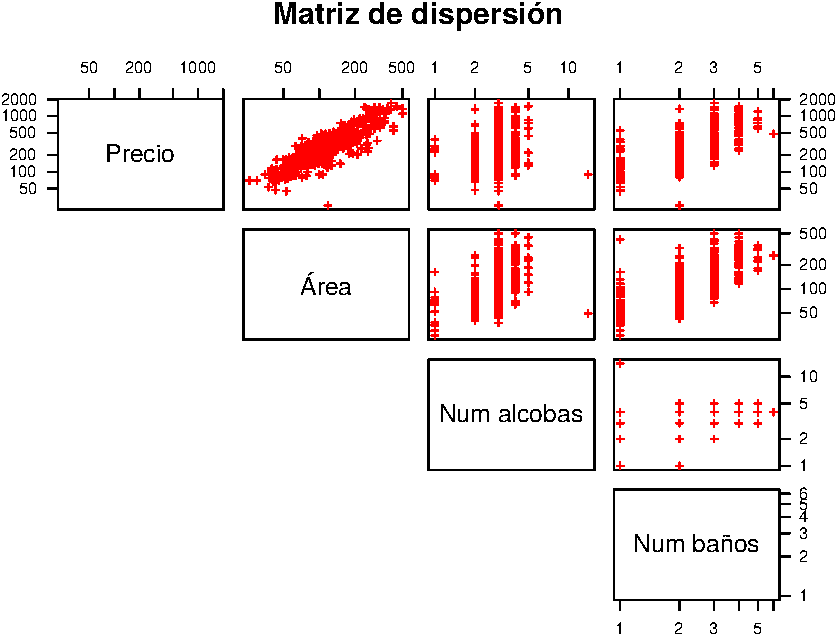
\includegraphics{Graficos_con_R_files/figure-latex/ex2pairs-1.pdf}
\caption{\label{fig:ex2pairs}Matriz de dispersión modificando los parámetros
adicionales de la función pairs.}
\end{figure}

\subsection*{Ejemplo}\label{ejemplo-15}


Construir una matriz de dispersión con las variables precio, área y
avaluo para apartamentos que cumplan la condición
\(100 m^2 < area < 130 m^2\). Adicionalmente, se deben diferenciar los
apartamentos sin parqueadero con color rojo y los apartamentos con
parqueadero con color verde.

Para crear una matriz de dispersión se puede tambien usar la base de
datos original llamada \texttt{datos} que contiene todas las variables y
usar una fórmula con la ayuda del operador \texttt{\textasciitilde{}}
para indicar las variables de interés. La fórmula \textbf{NO} debe
contener nada del lado izquierdo mientras que en el lado derecho se
colocan todas las variables a considerar en la matriz de dispersión, por
esta razón es que en el códido mostrado abajo se inicia con la
instrucción \texttt{\textasciitilde{}\ precio\ +\ mt2\ +\ avaluo}. Para
incluir condiciones se usa el parámetro \texttt{subset} de la siguiente
manera:
\texttt{subset=mt2\ \textgreater{}\ 100\ \&\ mt2\ \textless{}\ 130}. A
continuación el código completo para construir la matriz de dispersión
solicitada.

\begin{Shaded}
\begin{Highlighting}[]
\NormalTok{col1 <-}\StringTok{ }\KeywordTok{ifelse}\NormalTok{(datos$parqueadero ==}\StringTok{ 'no'}\NormalTok{, }\StringTok{'red'}\NormalTok{, }\StringTok{'green3'}\NormalTok{)}
\KeywordTok{pairs}\NormalTok{(~}\StringTok{ }\NormalTok{precio +}\StringTok{ }\NormalTok{mt2 +}\StringTok{ }\NormalTok{avaluo, }\DataTypeTok{data=}\NormalTok{datos,}
      \DataTypeTok{lower.panel=}\OtherTok{NULL}\NormalTok{, }\DataTypeTok{col=}\NormalTok{col1,}
      \DataTypeTok{subset=}\NormalTok{mt2 >}\StringTok{ }\DecValTok{100} \NormalTok{&}\StringTok{ }\NormalTok{mt2 <}\StringTok{ }\DecValTok{130}\NormalTok{, }\DataTypeTok{pch=}\DecValTok{19}\NormalTok{, }\DataTypeTok{cex=}\FloatTok{0.8}\NormalTok{,}
      \DataTypeTok{main=}\StringTok{"Matriz de dispersión para aptos con }
\StringTok{      100 < área < 130 mt2"}\NormalTok{)}
\end{Highlighting}
\end{Shaded}

\begin{figure}[htbp]
\centering
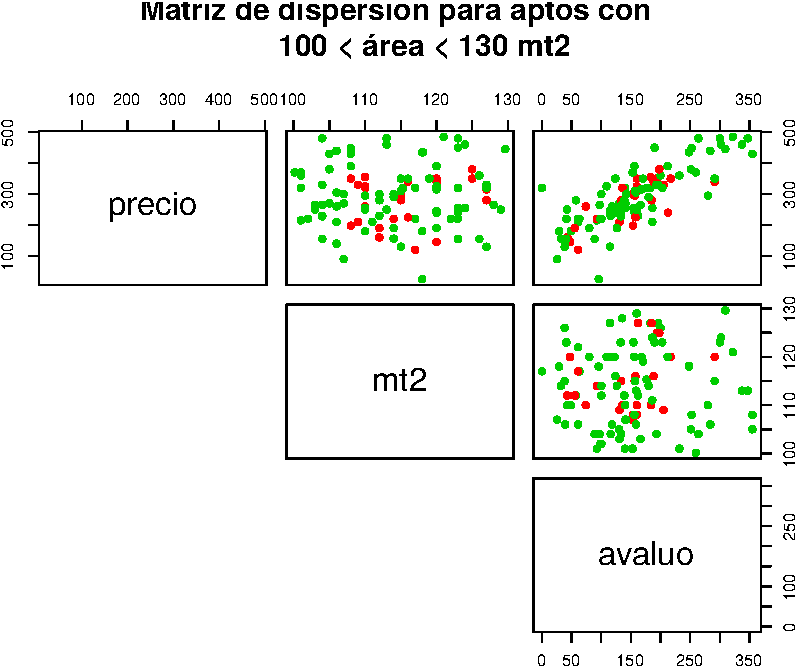
\includegraphics{Graficos_con_R_files/figure-latex/ex3pairs-1.pdf}
\caption{\label{fig:ex3pairs}Matriz de dispersión con un subconjunto de los
datos y con colores para identificar los puntos.}
\end{figure}

En la Figura \ref{fig:ex3pairs} se presenta la matriz de dispersión
solicitada, los puntos rojos representan los apartamento sin parqueadero
mientras que los puntos verdes son los apartamento que si tienen
parqueadero.

\subsection*{Ejemplo}\label{ejemplo-16}


¿Es posible agregar una leyenda a una matriz de dispersión?

Claro que es posible, se construye la matriz de dispersión y se deja en
el lienzo del dibujo un espacio para colocar la leyenda. A continuación
se muestra un ejemplo disponible en
\href{http://stackoverflow.com/questions/14948852/how-to-use-the-pairs-function-combined-with-layout-in-r}{Stackoverflow}.
A continuación se muestra el código para el ejemplo y en la Figura
\ref{fig:expairs} se presenta el resultado.

\begin{Shaded}
\begin{Highlighting}[]
\KeywordTok{pairs}\NormalTok{(iris[}\DecValTok{1}\NormalTok{:}\DecValTok{4}\NormalTok{], }\DataTypeTok{main=}\StringTok{"Anderson's Iris Data -- 3 species"}\NormalTok{,}
      \DataTypeTok{pch=}\DecValTok{21}\NormalTok{, }\DataTypeTok{bg=}\KeywordTok{c}\NormalTok{(}\StringTok{"red"}\NormalTok{, }\StringTok{"green3"}\NormalTok{, }\StringTok{"blue"}\NormalTok{)[iris$Species],}
      \DataTypeTok{oma=}\KeywordTok{c}\NormalTok{(}\DecValTok{4}\NormalTok{, }\DecValTok{4}\NormalTok{, }\DecValTok{6}\NormalTok{, }\DecValTok{12}\NormalTok{))}
\KeywordTok{par}\NormalTok{(}\DataTypeTok{xpd=}\OtherTok{TRUE}\NormalTok{)}
\KeywordTok{legend}\NormalTok{(}\FloatTok{0.85}\NormalTok{, }\FloatTok{0.7}\NormalTok{, }\KeywordTok{as.vector}\NormalTok{(}\KeywordTok{unique}\NormalTok{(iris$Species)), }\DataTypeTok{bty=}\StringTok{'n'}\NormalTok{,}
       \DataTypeTok{fill=}\KeywordTok{c}\NormalTok{(}\StringTok{"red"}\NormalTok{, }\StringTok{"green3"}\NormalTok{, }\StringTok{"blue"}\NormalTok{))}
\end{Highlighting}
\end{Shaded}

\begin{figure}[htbp]
\centering
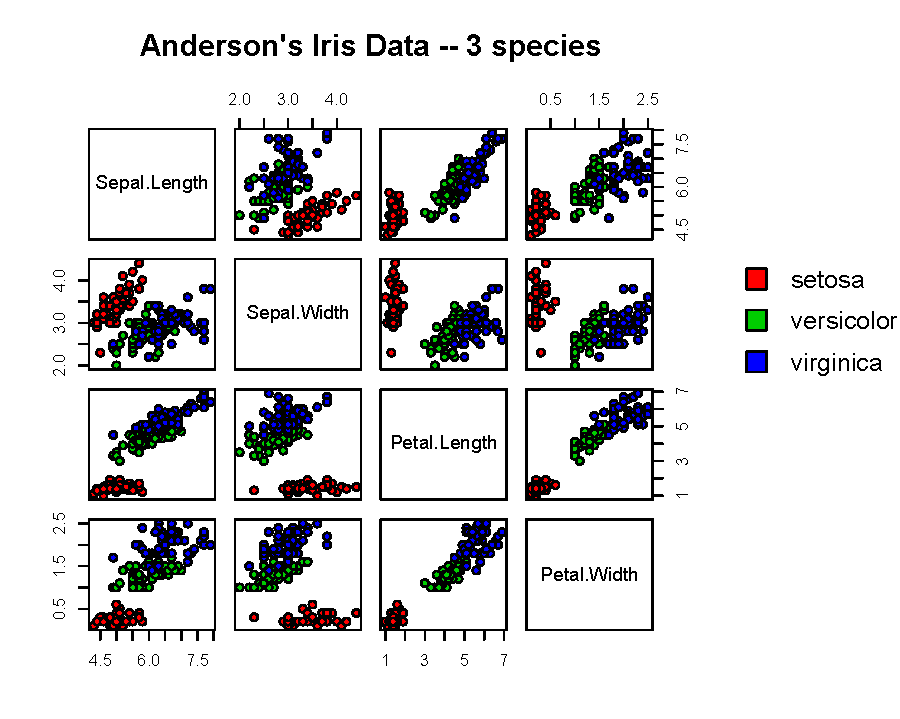
\includegraphics{Graficos_con_R_files/figure-latex/expairs-1.pdf}
\caption{\label{fig:expairs}Matriz de dispersión con leyenda.}
\end{figure}

\subsection*{Ejemplo}\label{ejemplo-17}


¿Es posible modificar el contenido de los páneles de una matriz de
dispersión?

Claro que es posible, para hacer esto se definen funciones que hagan lo
que se desea ver tanto en la diagonal como arriba y abajo de la misma.

Como ejemplo vamos a construir una matriz de dispersión que cumpla:

\begin{itemize}
\tightlist
\item
  sobre la diagonal un diagrama de dispersión para las variables
  involucradas y la recta de regresión ajustada,
\item
  en la diagonal un histograma para la variable,
\item
  debajo de la diagonal el coeficiente de correlación entre las
  variables involucradas y usando un tamaño de fuente proporcional a la
  fuerza de correlación.
\end{itemize}

Para obtener esta matriz de dispersión especial se definen a
continuación las funciones \texttt{panel.reg}, \texttt{panel.hist} y
\texttt{panel.cor}, a continuación el código utilizado. Luego se usa la
función \texttt{pairs} y se indica qué función debe actuar en cada uno
de los parámetros \texttt{upper.panel}, \texttt{diag.panel} y
\texttt{lower.panel}.

\begin{Shaded}
\begin{Highlighting}[]
\CommentTok{# Función para dibujar los puntos y agregar la recta de regresión}
\NormalTok{panel.reg <-}\StringTok{ }\NormalTok{function (x, y) }
\NormalTok{\{}
  \KeywordTok{points}\NormalTok{(x, y, }\DataTypeTok{pch=}\DecValTok{20}\NormalTok{)}
  \KeywordTok{abline}\NormalTok{(}\KeywordTok{lm}\NormalTok{(y ~}\StringTok{ }\NormalTok{x), }\DataTypeTok{lwd=}\DecValTok{2}\NormalTok{, }\DataTypeTok{col=}\StringTok{'dodgerblue2'}\NormalTok{)}
\NormalTok{\}}

\CommentTok{# Función para crear el histograma}
\NormalTok{panel.hist <-}\StringTok{ }\NormalTok{function(x, ...)}
\NormalTok{\{}
  \NormalTok{usr <-}\StringTok{ }\KeywordTok{par}\NormalTok{(}\StringTok{"usr"}\NormalTok{); }\KeywordTok{on.exit}\NormalTok{(}\KeywordTok{par}\NormalTok{(usr))}
  \KeywordTok{par}\NormalTok{(}\DataTypeTok{usr =} \KeywordTok{c}\NormalTok{(usr[}\DecValTok{1}\NormalTok{:}\DecValTok{2}\NormalTok{], }\DecValTok{0}\NormalTok{, }\FloatTok{1.5}\NormalTok{) )}
  \NormalTok{h <-}\StringTok{ }\KeywordTok{hist}\NormalTok{(x, }\DataTypeTok{plot =} \OtherTok{FALSE}\NormalTok{)}
  \NormalTok{breaks <-}\StringTok{ }\NormalTok{h$breaks; nB <-}\StringTok{ }\KeywordTok{length}\NormalTok{(breaks)}
  \NormalTok{y <-}\StringTok{ }\NormalTok{h$counts; y <-}\StringTok{ }\NormalTok{y/}\KeywordTok{max}\NormalTok{(y)}
  \KeywordTok{rect}\NormalTok{(breaks[-nB], }\DecValTok{0}\NormalTok{, breaks[-}\DecValTok{1}\NormalTok{], y, }\DataTypeTok{col=}\StringTok{"dodgerblue2"}\NormalTok{, ...)}
\NormalTok{\}}

\CommentTok{# Función para obtener la correlación}
\NormalTok{panel.cor <-}\StringTok{ }\NormalTok{function(x, y, }\DataTypeTok{digits=}\DecValTok{2}\NormalTok{, }\DataTypeTok{prefix=}\StringTok{""}\NormalTok{, cex.cor)}
\NormalTok{\{}
  \NormalTok{usr <-}\StringTok{ }\KeywordTok{par}\NormalTok{(}\StringTok{"usr"}\NormalTok{); }\KeywordTok{on.exit}\NormalTok{(}\KeywordTok{par}\NormalTok{(usr))}
  \KeywordTok{par}\NormalTok{(}\DataTypeTok{usr =} \KeywordTok{c}\NormalTok{(}\DecValTok{0}\NormalTok{, }\DecValTok{1}\NormalTok{, }\DecValTok{0}\NormalTok{, }\DecValTok{1}\NormalTok{))}
  \NormalTok{r <-}\StringTok{ }\KeywordTok{abs}\NormalTok{(}\KeywordTok{cor}\NormalTok{(x, y))}
  \NormalTok{txt <-}\StringTok{ }\KeywordTok{format}\NormalTok{(}\KeywordTok{c}\NormalTok{(r, }\FloatTok{0.123456789}\NormalTok{), }\DataTypeTok{digits=}\NormalTok{digits)[}\DecValTok{1}\NormalTok{]}
  \NormalTok{txt <-}\StringTok{ }\KeywordTok{paste}\NormalTok{(prefix, txt, }\DataTypeTok{sep=}\StringTok{""}\NormalTok{)}
  \NormalTok{if(}\KeywordTok{missing}\NormalTok{(cex.cor)) cex <-}\StringTok{ }\FloatTok{0.8}\NormalTok{/}\KeywordTok{strwidth}\NormalTok{(txt)}
  \KeywordTok{text}\NormalTok{(}\FloatTok{0.5}\NormalTok{, }\FloatTok{0.5}\NormalTok{, txt, }\DataTypeTok{cex =} \NormalTok{cex *}\StringTok{ }\NormalTok{r)}
\NormalTok{\}}

\KeywordTok{pairs}\NormalTok{(datos.num,}
      \DataTypeTok{upper.panel =} \NormalTok{panel.reg,}
      \DataTypeTok{diag.panel =} \NormalTok{panel.hist,}
      \DataTypeTok{lower.panel =} \NormalTok{panel.cor)}
\end{Highlighting}
\end{Shaded}

\begin{figure}[htbp]
\centering
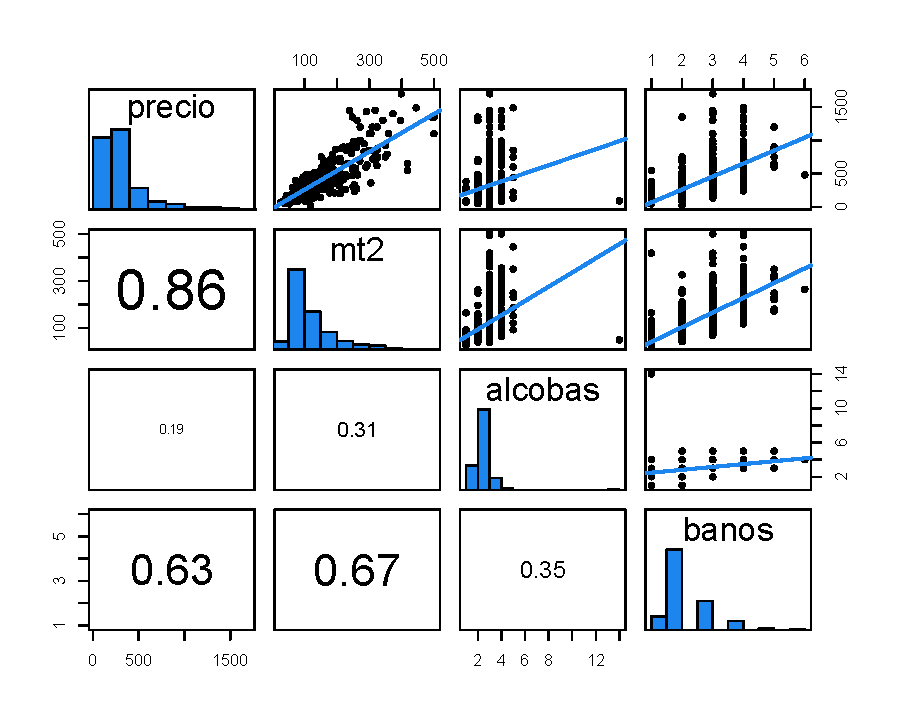
\includegraphics{Graficos_con_R_files/figure-latex/exmod1pairs-1.pdf}
\caption{\label{fig:exmod1pairs}Matriz de dispersión con páneles
modificados.}
\end{figure}

En la Figura \ref{fig:exmod1pairs} se presenta la matriz de dispersión
con las modificaciones en cada uno de los páneles. Cualquier usuario
puede modificar las funciones \texttt{panel.reg}, \texttt{panel.hist} y
\texttt{panel.cor} para personalizar la apariencia de los contenidos.

La función \texttt{panel.smooth} está disponible en \proglang{R} para
que el usuario pueda incluir arriba o abajo de la diagonal un diagrama
de dispersión con una línea resultado de un ajuste suavizado. Abajo se
muestra el código de cómo incluir la función \texttt{panel.smooth} y en
la Figura \ref{fig:exmod2pairs} se muestra gráfico obtenido.

\begin{Shaded}
\begin{Highlighting}[]
\KeywordTok{pairs}\NormalTok{(datos.num,}
      \DataTypeTok{upper.panel =} \NormalTok{panel.reg,}
      \DataTypeTok{diag.panel =} \NormalTok{panel.hist,}
      \DataTypeTok{lower.panel =} \NormalTok{panel.smooth)}
\end{Highlighting}
\end{Shaded}

\begin{figure}[htbp]
\centering
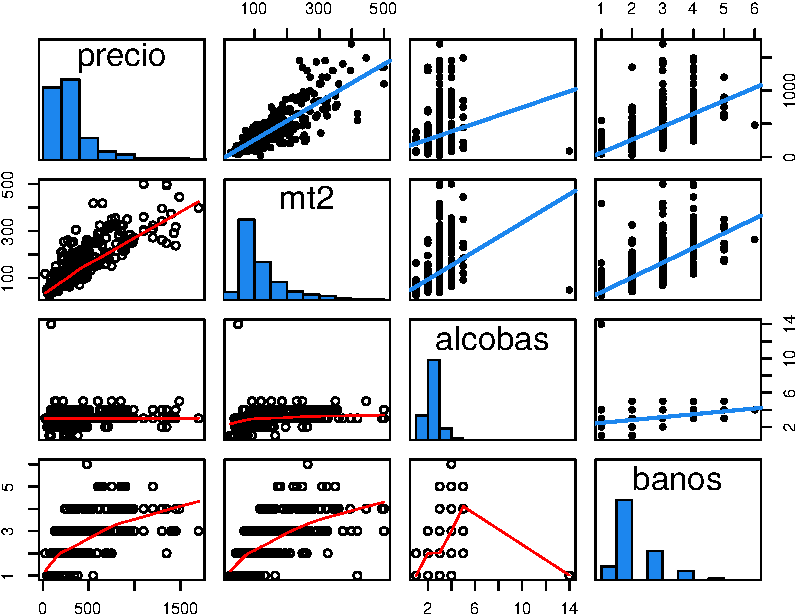
\includegraphics{Graficos_con_R_files/figure-latex/exmod2pairs-1.pdf}
\caption{\label{fig:exmod2pairs}Matriz de dispersión usando la función
panel.smooth.}
\end{figure}

\section{\texorpdfstring{Función \texttt{contour} \index{contour}
\index{gráfico de contornos}}{Función contour  }}\label{funcion-contour}

\cleardoublepage 

\appendix \addcontentsline{toc}{chapter}{\appendixname}


\chapter{More to Say}\label{more-to-say}

Yeah! I have finished my book, but I have more to say about some topics.
Let me explain them in this appendix.

To know more about \textbf{bookdown}, see \url{https://bookdown.org}.

\bibliography{packages,book}

\backmatter
\printindex

\end{document}
